\chapter{随机变量的分布}
\label{chap:random-variables}

掷两枚骰子，赌局只看点数之和；从一批产品里抽两件检验，质检员只记次品有几件；在窗口前排队，顾客只在意等了几分钟。试验的结果本身可能很复杂，我们真正关心的却往往是由结果算出的一个数。这个数事先不知道，但它可能取哪些值、落在各个范围里的概率有多大，是可以说清楚的。

把这些问题写下来，就是本章要处理的几件事。点数之和等于$7$的概率是多少？次品不超过一件的概率是多少？等待时间落在$1$到$2$分钟之间的概率是多少？反过来，给定$90\%$这样的比例，多长的等待才能覆盖九成顾客？还有一个更基本的问题：用什么样的一张表或一个函数，才能一次记下所有这些答案？

第~\ref{chap:classical-probability}章在有限个等可能结果上计算事件的概率。本章先把“由结果算出的数”写成样本空间上的函数，即随机变量，并把注意力从具体结果转到它的取值规律，即分布。接着用分布函数统一记录实轴上的累计概率，再分别用概率质量和密度给出离散取值与连续取值时更直接的表示。分位数从反方向读分布函数，回答“给定概率，阈值在哪里”。最后检查这些表示各自的适用范围：有些分布既不能写成一张概率表，也没有密度，只有分布函数始终可用。

全章反复使用几个能手算的模型：骰子、不放回抽检、首次掷出六点所需的次数，以及以分钟计的等待时间。读者只需要第~\ref{chap:classical-probability}章的计数与条件概率，以及卷一的级数与积分。

\section{随机变量}
\label{sec:rvd-random-variables}

掷一枚骰子，样本空间是$\Omega=\{1,2,3,4,5,6\}$。如果关心点数，就把结果$\omega$记成数$\omega$；如果只关心奇偶，就把偶数结果记成$1$、奇数结果记成$0$。两种记录面对的是同一次试验，区别只在于“结果怎样变成数”。这种记录规则怎样精确表述，它取各个值的概率又怎样从结果的概率得到？

\paragraph{结果到数值的映射}
图~\ref{fig:rvd-die-maps}画出了两种记录。中间一行是六个结果，向上的箭头把每个结果送到它的点数，向下的箭头把三个偶数结果送到$1$、三个奇数结果送到$0$。两种记录都是从$\Omega$到实数的函数，只是第二个函数把不同的结果合并到了同一个值。

\begin{BookInlineFigure}
  \centering
  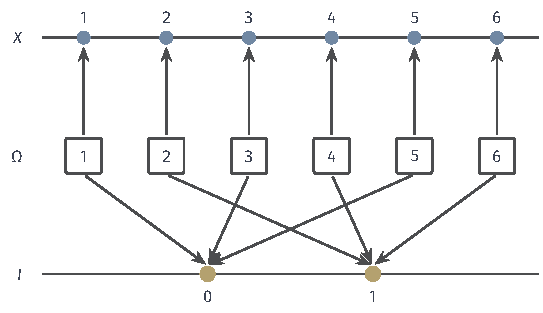
\includegraphics[width=92mm]{figures/07-probability/01-elementary-probability/tikz/rvd-die-maps/figure.pdf}
  \caption{同一次掷骰上的两个随机变量。中间一行是样本空间$\Omega$的六个结果。向上的箭头是点数$X$，六个结果送到六个不同的值（蓝点）；向下的箭头是奇偶记录$I$，三个奇数结果都送到$0$，三个偶数结果都送到$1$（黄点）。}
  \label{fig:rvd-die-maps}
\end{BookInlineFigure}

把这种规则一般地写出来，就得到随机变量。它的定义只用到样本空间和函数，概率在下一步才进入。

\begin{definition}[随机变量]
\label{def:rvd-random-variable}
设$\Omega$是一个试验的样本空间。函数$X:\Omega\to\mathbb{R}$称为\term{随机变量}（random variable）。对实数集的子集$B$，记
\begin{equation}
  \{X\in B\}=\{\omega\in\Omega:X(\omega)\in B\},
  \label{eq:rvd-preimage}
\end{equation}
它是由满足$X(\omega)\in B$的结果组成的事件，其概率记作$\mathbb{P}(X\in B)$。
\end{definition}

常用的事件有简写：$\{X\leq x\}$表示$B=(-\infty,x]$，$\{X=x\}$表示$B=\{x\}$，$\{a<X\leq b\}$表示$B=(a,b]$。在骰子的例子里，点数记录是$X(\omega)=\omega$，奇偶记录是
\[
  I(\omega)=\begin{cases}1,&\omega\in\{2,4,6\},\\0,&\omega\in\{1,3,5\}.\end{cases}
\]
于是$\{I=1\}=\{2,4,6\}$，$\{X\leq 2\}=\{1,2\}$，它们都是$\Omega$的子集，也就是第~\ref{chap:classical-probability}章意义下的事件。

一般地，对事件$A$，在$A$上取$1$、在$A$外取$0$的函数记作$\mathbf{1}_{A}$，称为$A$的\term{指示函数}（indicator function）。奇偶记录就是$I=\mathbf{1}_{\{2,4,6\}}$。指示函数把事件和随机变量联系起来：$\{\mathbf{1}_{A}=1\}=A$，所以$\mathbb{P}(\mathbf{1}_{A}=1)=\mathbb{P}(A)$。事件可以看成只取$0$和$1$的随机变量。

\paragraph{随机变量、实现值与事件}
“随机变量”这个名字容易误导：$X$本身是一个完全确定的函数，随机的是哪个结果$\omega$出现。试验做完，结果$\omega$确定，$X$就取一个具体的数$x=X(\omega)$，称为$X$的一个\term{实现值}（realization）。我们用大写字母表示随机变量，小写字母表示它的取值。

三种对象要分清。$X$是规则，在试验之前就已给定；$\{X\leq 2\}$是事件，是一个由结果组成的集合，事先可以问它的概率；“这次掷出$x=5$”是一次实现，事后才知道。说“$\mathbb{P}(X\leq 2)=1/3$”是在谈事件，说“$x=5>2$，所以事件$\{X\leq2\}$这次没有发生”是在用实现值检验事件。

\paragraph{由结果的概率得到取值的概率}
骰子公平时，每个结果的概率是$1/6$。要算$I$取$1$的概率，就把被送到$1$的结果的概率加起来：
\[
  \mathbb{P}(I=1)=\mathbb{P}(\{2,4,6\})=\tfrac16+\tfrac16+\tfrac16=\tfrac12 .
\]
可以把$\mathbb{P}$想成单位质量在六个结果上的分配，每个结果分到$1/6$。随机变量沿箭头把每个结果的质量搬到它的取值上，同一个取值收到的质量相加。$X$把六份质量分别搬到$1,\dots,6$，$I$把三份搬到$0$、三份搬到$1$。

同一个函数配上不同的概率，搬运的结果就不同。设骰子被做了手脚，$\mathbb{P}(\{6\})=1/2$，其余五面各为$1/10$。函数$I$没有变，但
\[
  \mathbb{P}(I=1)=0.1+0.1+0.5=0.7 .
\]
所以随机变量取值的概率规律由两样东西共同决定：结果到数值的规则$X$，以及结果上的概率$\mathbb{P}$。

\paragraph{无限多个结果}
等待时间可以是任何非负实数，样本空间$\Omega=[0,\infty)$有无穷多个结果，第~\ref{chap:classical-probability}章的计数比不再适用。本部分对这类试验直接规定区间事件的概率：例如规定等待超过$t$分钟的概率，再由加减得到其他区间的概率。具体的规定方式由下一节的分布函数和第~\ref{sec:rvd-mass-density}节的密度给出。

这样做时只对区间及其有限并谈概率，对取有限或可数个值的变量则对取值的任意子集谈概率。一般样本空间上哪些集合可以赋予概率、怎样保证各种规定彼此相容，在第~\ref{chap:probability-spaces}章统一处理。本部分用到的事件都是上面这些具体的集合，不会遇到困难。

\paragraph{同一次试验的不同记录}
同一次试验可以同时定义许多随机变量。掷两枚骰子，样本空间是$36$个等可能的有序对$\omega=(i,j)$。记点数之和为$S(\omega)=i+j$，较大的点数为$M(\omega)=\max\{i,j\}$。两者都是$\Omega$上的函数，记录的是同一次投掷的不同侧面。

事件$\{S=7\}$由反对角线上的六个结果组成，所以$\mathbb{P}(S=7)=6/36$。事件$\{M=4\}$由“较大者恰为$4$”的结果组成：$(4,1),\dots,(4,4)$与$(1,4),(2,4),(3,4)$，共$7$个，所以$\mathbb{P}(M=4)=7/36$。图~\ref{fig:rvd-two-dice}(a)用圆点和方框标出了这两个事件，$(3,4)$和$(4,3)$同时属于两者。

\begin{BookInlineFigure}
  \centering
  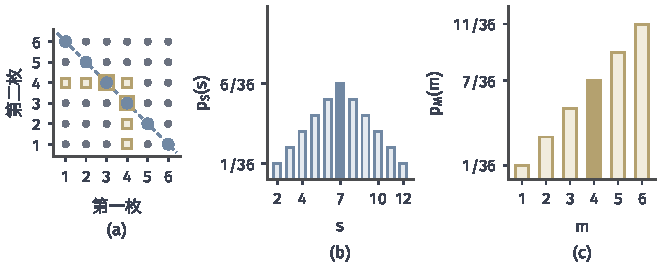
\includegraphics[width=112mm]{figures/07-probability/01-elementary-probability/matplotlib/rvd-two-dice/figure.pdf}
  \caption{两枚公平骰子上的两个随机变量。(a)$36$个等可能结果，蓝色圆点（沿虚线）是事件$\{S=7\}$，黄色方框是事件$\{M=4\}$，两个结果同时属于二者。(b)点数之和$S$取各值的概率，深色柱是$s=7$。(c)较大点数$M$取各值的概率，深色柱是$m=4$。}
  \label{fig:rvd-two-dice}
\end{BookInlineFigure}

对每个取值都这样计数，就得到图~\ref{fig:rvd-two-dice}(b)(c)。和为$s$的结果沿一条反对角线排列，条数先增后减，于是
\begin{equation}
  \mathbb{P}(S=s)=\frac{6-\lvert s-7\rvert}{36},\qquad s=2,3,\dots,12 .
  \label{eq:rvd-dice-sum}
\end{equation}
较大点数先用累计事件计数更方便：$\{M\leq m\}$要求两枚骰子都不超过$m$，有$m^{2}$个结果。$\{M=m\}$是$\{M\leq m\}$去掉$\{M\leq m-1\}$，所以
\[
  \mathbb{P}(M=m)=\frac{m^{2}-(m-1)^{2}}{36}=\frac{2m-1}{36},\qquad m=1,\dots,6 .
\]
两张表的概率各自加起来都等于$1$。

两个记录来自同一次投掷，彼此并不无关。知道$M=1$，就只能是$(1,1)$，于是$S=2$。这种同时考察多个随机变量的问题由第~\ref{chap:random-vectors}章处理，本章每次只看一个随机变量。

\paragraph{分布}
算出$\mathbb{P}(S=s)$之后，回答“$S$落在某个范围的概率”就不再需要回到$36$个结果：例如$\mathbb{P}(S\geq 10)=(3+2+1)/36=1/6$。我们只关心一个随机变量本身时，需要的正是这种“取值落在哪里、概率多大”的规律。

\begin{definition}[分布]
\label{def:rvd-distribution}
随机变量$X$的\term{分布}（probability distribution）是对实数集的子集$B$给出概率的规则
\begin{equation}
  P_X(B)=\mathbb{P}(X\in B)=\mathbb{P}(\{\omega\in\Omega:X(\omega)\in B\}).
  \label{eq:rvd-distribution}
\end{equation}
本部分中$B$取区间及其有限并；$X$只取有限或可数个值时，$B$可取这些值组成的任意集合。
\end{definition}

按搬运质量的图景，$\mathbb{P}$是单位质量在样本空间上的分配，$P_X$是这些质量被$X$搬到实轴之后的分配。分布只记录质量最后停在哪里，不再记录它从哪个结果搬来。这既是分布的用处，也是它的局限：凡是只涉及$X$一个变量取值的概率问题，分布都能回答；凡是涉及“哪个结果产生了这个值”的问题，分布无能为力。

\paragraph{分布本身也是概率}
$P_X$满足第~\ref{chap:classical-probability}章概率的基本规则，只是它作用在实数集的子集上，而不是$\Omega$的子集上。原因在于取原像与集合运算可以交换次序。对实数集的子集$B_1,B_2$，结果$\omega$属于$\{X\in B_1\cup B_2\}$，当且仅当$X(\omega)$落在$B_1$或$B_2$中，即$\omega$属于两个事件之一，所以
\[
  \{X\in B_1\cup B_2\}=\{X\in B_1\}\cup\{X\in B_2\}.
\]
同理，$\{X\notin B\}$是事件$\{X\in B\}$在$\Omega$中的补。

若$B_1$与$B_2$不相交，没有哪个结果能让$X(\omega)$同时落在两者中，两个事件互斥。由概率的可加性，
\[
  P_X(B_1\cup B_2)=P_X(B_1)+P_X(B_2).
\]
再加上$P_X(B)\geq0$和$P_X(\mathbb{R})=\mathbb{P}(\Omega)=1$，$P_X$就是实轴上的一个概率分配。此后只研究$X$时，可以把取值的集合当作新的样本空间，忘掉原来的$\Omega$。

新的样本空间上的概率通常不再是等可能的。两枚骰子的$36$个结果等可能，但点数之和的$11$个取值概率各不相同，式~\eqref{eq:rvd-dice-sum}中$7$的概率是$2$的六倍。在取值集合$\{2,\dots,12\}$上直接“数有利取值”会得出错误答案，这正是第~\ref{chap:classical-probability}章强调的：把基本结果合并之后，不能继续把合并后的类别当作等可能。

\paragraph{相同分布不等于相同取值}
在公平骰子上再定义$Y(\omega)=7-\omega$，即骰子底面的点数。$X$和$Y$在每个结果上都不相等，因为$X(\omega)=Y(\omega)$要求$\omega=3.5$。但$Y$取每个值$k$的概率是
\[
  \mathbb{P}(Y=k)=\mathbb{P}(\{7-k\})=\tfrac16,\qquad k=1,\dots,6,
\]
与$X$完全相同。图~\ref{fig:rvd-same-law}(a)逐个结果画出两个取值，(b)画出两者取各值的概率。

\begin{BookInlineFigure}
  \centering
  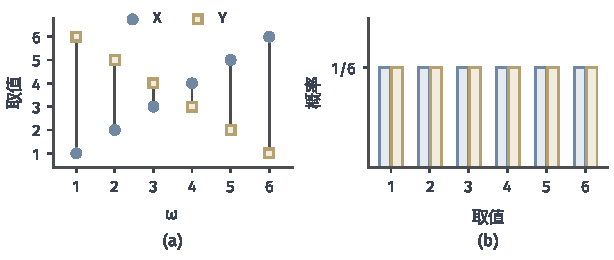
\includegraphics[width=104mm]{figures/07-probability/01-elementary-probability/matplotlib/rvd-same-law/figure.pdf}
  \caption{分布相同而取值不同。公平骰子上，$X(\omega)=\omega$（蓝点）与$Y(\omega)=7-\omega$（黄框）。(a)每个结果上两者的取值，竖线连接同一结果的两个值，没有一个结果使二者相等；(b)两者取$1,\dots,6$的概率都是$1/6$。}
  \label{fig:rvd-same-law}
\end{BookInlineFigure}

若$P_X=P_Y$，即对所有$B$都有$\mathbb{P}(X\in B)=\mathbb{P}(Y\in B)$，就说$X$与$Y$\term{同分布}（identically distributed）。同分布只是说两个变量“单独看”无法区分，不是说它们相等。这个例子里$X+Y$恒等于$7$，但仅凭两个分布无法知道这一点：若把$Y$换成另一枚独立骰子的点数，两个分布照旧，$X+Y$却会取$2$到$12$之间的各种值。表~\ref{tab:rvd-three-objects}总结了三个对象的区别。

\begin{BookInlineTable}
  \centering
  \begin{tabular}{lll}
    \toprule
    对象 & 是什么 & 骰子中的例子\\
    \midrule
    随机变量$X$ & $\Omega$上的函数 & $X(\omega)=\omega$\\
    实现值$x$ & 一次试验得到的数 & 这次掷出$x=5$\\
    分布$P_X$ & 实轴子集上的概率 & 每个点数概率$1/6$\\
    \bottomrule
  \end{tabular}
  \caption{随机变量、实现值与分布。前者是规则，中者是一次结果，后者是取值的概率规律；$X$与$7-X$是两个不同的规则，分布却相同。}
  \label{tab:rvd-three-objects}
\end{BookInlineTable}

\paragraph{随机变量的函数}
有了随机变量$X$和实函数$g$，复合$g(X)$，即$\omega\mapsto g(X(\omega))$，仍是$\Omega$上的函数，因而仍是随机变量。前面的$Y=7-X$就是$g(x)=7-x$的情形。抽检中，若抽两件、次品数为$X$，则合格品数是$2-X$，也属于这种情形。

$g(X)$的分布可以只用$X$的分布求出。事件$\{g(X)\in B\}$就是$\{X\in g^{-1}(B)\}$，其中$g^{-1}(B)$是被$g$送进$B$的$x$组成的集合。$X$只取有限或可数个值时，这给出
\begin{equation}
  \mathbb{P}(g(X)=y)=\sum_{x:\,g(x)=y}\mathbb{P}(X=x),
  \label{eq:rvd-function-pmf}
\end{equation}
即把被$g$送到同一个$y$的那些$x$的概率加起来。

下面用公平骰子的点数演示，取$g(x)=(x-3)^{2}$。$X=1,\dots,6$分别被送到$4,1,0,1,4,9$，其中$1$和$4$各收到两个点数。由式~\eqref{eq:rvd-function-pmf}，$Z=(X-3)^{2}$取各值的概率是
\[
  \mathbb{P}(Z=0)=\tfrac16,\quad \mathbb{P}(Z=1)=\tfrac26,\quad \mathbb{P}(Z=4)=\tfrac26,\quad \mathbb{P}(Z=9)=\tfrac16 .
\]
计算中没有回到样本空间，只用了$X$取各值的概率。取值连续变化的变量经过函数后分布怎样变化，需要换元等工具，由第~\ref{chap:random-variable-transformations}章处理。


\section{分布函数}
\label{sec:rvd-distribution-functions}

分布要对许多集合给出概率。骰子只有六个取值，列一张表就够了；等待时间可以取任何非负实数，不可能把每个区间的概率逐一列出。能不能用一个实变量的函数记下全部信息？

\paragraph{累计到阈值的概率}
设想沿实轴从左向右移动一个阈值$x$，每到一处就问：取值不超过$x$的概率有多大？按质量的图景，这是阈值左侧（含阈值本身）累积的质量。阈值移动时，这个数只增不减，从$0$开始，最后到$1$。

\begin{definition}[分布函数]
\label{def:rvd-cdf}
随机变量$X$的\term{分布函数}（cumulative distribution function）定义为
\begin{equation}
  F_X(x)=\mathbb{P}(X\leq x),\qquad x\in\mathbb{R}.
  \label{eq:rvd-cdf}
\end{equation}
\end{definition}

分布函数对每个实数$x$都有定义，不论$X$实际取哪些值。只要知道它，左开右闭区间的概率就能算出。设$a<b$，事件$\{X\leq b\}$是互斥的$\{X\leq a\}$与$\{a<X\leq b\}$之并，由可加性
\[
  \mathbb{P}(X\leq b)=\mathbb{P}(X\leq a)+\mathbb{P}(a<X\leq b),
\]
移项得到
\begin{equation}
  \mathbb{P}(a<X\leq b)=F_X(b)-F_X(a).
  \label{eq:rvd-interval}
\end{equation}
区间取左开右闭，正好与定义中的“$\leq$”配套：$\{X\leq a\}$含$a$，减去之后右边的区间就不含$a$。

\paragraph{抽检中的次品数}
一批$5$件产品中有$2$件次品，不放回地随机抽取$2$件，记次品数为$X$。按第~\ref{chap:classical-probability}章的计数，无序抽法共$\binom52=10$种，等可能。两件都合格有$\binom32=3$种，一件次品一件合格有$2\times3=6$种，两件都是次品有$1$种。于是
\[
  \mathbb{P}(X=0)=0.3,\quad \mathbb{P}(X=1)=0.6,\quad \mathbb{P}(X=2)=0.1 .
\]

现在让阈值$x$扫过实轴。$x<0$时没有任何可能取值不超过$x$；$0\leq x<1$时只有取值$0$满足；$1\leq x<2$时取值$0$和$1$满足；$x\geq2$时全部满足。所以
\begin{equation}
  F_X(x)=\begin{cases}
    0,&x<0,\\
    0.3,&0\leq x<1,\\
    0.9,&1\leq x<2,\\
    1,&x\geq 2.
  \end{cases}
  \label{eq:rvd-inspection-cdf}
\end{equation}
图~\ref{fig:rvd-inspection-cdf}以$x=1.5$为例：(a)中红线左侧的柱子是被累计的质量，(b)中红点是它们的和$F_X(1.5)=0.9$。

\begin{BookInlineFigure}
  \centering
  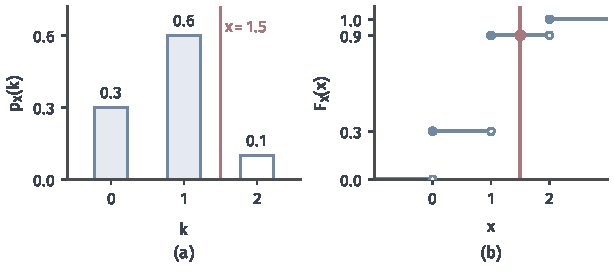
\includegraphics[width=104mm]{figures/07-probability/01-elementary-probability/matplotlib/rvd-inspection-cdf/figure.pdf}
  \caption{抽检次品数$X$的分布函数。(a)$X$取$0,1,2$的概率，红线是阈值$x=1.5$，左侧浅蓝柱被累计，右侧白柱不计；(b)分布函数，实心点是函数值，空心点是从左侧逼近的极限。红点$F_X(1.5)=0.3+0.6=0.9$。}
  \label{fig:rvd-inspection-cdf}
\end{BookInlineFigure}

$F_X$是阶梯函数：在两个可能取值之间，阈值移动不会越过新的质量，函数保持水平；阈值越过一个可能取值时，函数跳升，跳升的高度正是该处的概率。注意每个台阶的左端是实心点：$F_X(1)=0.9$，因为$\{X\leq1\}$包含$X=1$。

\paragraph{等待时间}
等待时间$T$（单位：分钟）不能列表，我们直接用分布函数给出模型：
\begin{equation}
  F_T(t)=\begin{cases}0,&t<0,\\1-\mathrm{e}^{-t},&t\geq0.\end{cases}
  \label{eq:rvd-waiting-cdf}
\end{equation}
它等价于规定“等待超过$t$分钟的概率是$\mathrm{e}^{-t}$”，等待越久越罕见。为什么这种形式适合描述等待，留到第~\ref{chap:common-distributions}章说明，这里只把它当作给定的模型。由式~\eqref{eq:rvd-interval}，等待$1$到$2$分钟的概率是
\[
  \mathbb{P}(1<T\leq2)=(1-\mathrm{e}^{-2})-(1-\mathrm{e}^{-1})=\mathrm{e}^{-1}-\mathrm{e}^{-2}\approx0.2325 .
\]
等待超过$2$分钟的概率是$1-F_T(2)=\mathrm{e}^{-2}\approx0.1353$。

这条曲线处处连续，没有跳跃。与抽检的阶梯对比，可以预料：跳跃对应集中在单点的概率，而等待时间没有哪一个具体时刻带有正概率。下面把这个预料写成定理。

\paragraph{分布函数的性质}
阶梯函数和连续曲线看起来很不同，但它们有共同的骨架：单调不减，在每一点从右侧连续，两端分别趋于$0$和$1$，跳跃高度等于单点概率。先对取有限或可数个值的随机变量证明这些性质；用密度给出的模型在第~\ref{sec:rvd-mass-density}节核验，一般情形的依据在第~\ref{chap:probability-spaces}章给出。

设$X$只取值$x_1,x_2,\dots$（有限个或可数个，互不相同），记$q_i=\mathbb{P}(X=x_i)$，这些数非负，总和为$1$。取有限个值时，每个事件的概率就是其中各取值概率之和；取可数个值时，我们把这一点作为模型的规定：$\mathbb{P}(X\in B)$等于$x_i\in B$的那些$q_i$之和。非负项级数可以任意重排和分组而和不变，所以这样规定的概率同样满足可加性。于是
\[
  F_X(x)=\sum_{i:\,x_i\leq x}q_i .
\]

\begin{theorem}[分布函数的性质]
\label{thm:rvd-cdf-properties}
设随机变量$X$只取有限或可数个值，$F=F_X$。则
\begin{enumerate}
  \item 单调不减：$x<y$时$F(x)\leq F(y)$；
  \item 右连续：对每个$x$，$\lim_{h\downarrow0}F(x+h)=F(x)$；
  \item 两端极限：$\lim_{x\to-\infty}F(x)=0$，$\lim_{x\to+\infty}F(x)=1$；
  \item 左极限存在，并且
  \begin{equation}
    F(x^{-})=\lim_{h\downarrow0}F(x-h)=\mathbb{P}(X<x),\qquad F(x)-F(x^{-})=\mathbb{P}(X=x).
    \label{eq:rvd-jump}
  \end{equation}
\end{enumerate}
\end{theorem}

\begin{proof}
单调性：$x<y$时，满足$x_i\leq x$的下标都满足$x_i\leq y$，后者的和多出一些非负项，所以$F(x)\leq F(y)$。

其余三条都依靠同一个估计：总和为$1$的级数，尾部可以任意小。给定$\varepsilon>0$，取$N$使
\[
  \sum_{i>N}q_i<\varepsilon .
\]
这时只有前$N$个取值可能带来不小的概率，而有限个点总是离给定的点有正的距离。

右连续：$F(x+h)-F(x)$是落在$(x,x+h]$里的那些$q_i$之和。前$N$个取值中大于$x$的有有限个，记它们到$x$的最小距离为$\delta>0$（若没有这样的取值，取$\delta=1$）。当$0<h<\delta$时，前$N$个取值都不在$(x,x+h]$中，于是
\[
  0\leq F(x+h)-F(x)\leq\sum_{i>N}q_i<\varepsilon .
\]

两端极限：当$x$小于$x_1,\dots,x_N$中的最小者时，$F(x)$只含下标大于$N$的项，所以$F(x)<\varepsilon$。当$x$不小于其中最大者时，$F(x)$包含前$N$项，所以
\[
  F(x)\geq\sum_{i\leq N}q_i>1-\varepsilon .
\]
又$0\leq F\leq1$，两端极限分别为$0$和$1$。

左极限：$F(x)-F(x-h)$是落在$(x-h,x]$里的$q_i$之和，它等于$\mathbb{P}(X=x)$加上落在$(x-h,x)$里的那些项。与右连续的论证相同，$h$足够小时后者小于$\varepsilon$，所以
\[
  \lim_{h\downarrow0}\bigl(F(x)-F(x-h)\bigr)=\mathbb{P}(X=x).
\]
移项即得式~\eqref{eq:rvd-jump}中左极限的值$F(x)-\mathbb{P}(X=x)=\mathbb{P}(X<x)$。
\end{proof}

右连续而不一定左连续，原因在于“$\leq$”包含阈值本身。图~\ref{fig:rvd-jump-limits}放大了抽检例子在$x=1$处的跳跃。从右侧逼近时，阈值$1+1/n$与$1$之间没有可能取值，累计的总是$X=0$和$X=1$两份质量，函数值恒为$0.9=F(1)$。从左侧逼近时，阈值$1-1/n$还没有越过$1$，累计的只有$X=0$那一份，极限是$0.3$。两者之差$0.6$就是$X=1$的概率。

\begin{BookInlineFigure}
  \centering
  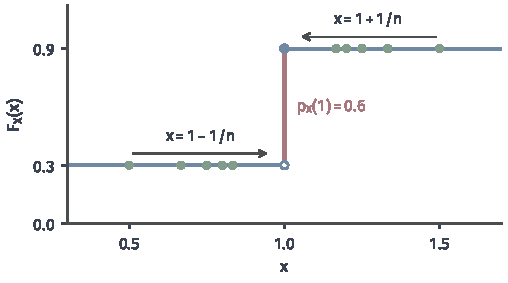
\includegraphics[width=86mm]{figures/07-probability/01-elementary-probability/matplotlib/rvd-jump-limits/figure.pdf}
  \caption{抽检次品数的分布函数在$x=1$处的两侧极限。绿点是阈值$1+1/n$与$1-1/n$（$n=2,\dots,6$）处的函数值：右侧一列恒为$0.9$，等于$F_X(1)$（实心点）；左侧一列恒为$0.3$，等于左极限（空心点）。红色竖线是跳跃高度$0.6=\mathbb{P}(X=1)$。}
  \label{fig:rvd-jump-limits}
\end{BookInlineFigure}

\paragraph{三条性质各管什么}
单调、右连续、两端极限这三条性质，每一条都排除了一类不可能是分布函数的函数。拿抽检例子对照，可以看清它们各自的作用。

单调不减保证区间概率非负：由式~\eqref{eq:rvd-interval}，$F(b)-F(a)$是概率，不能为负。右连续是“$\leq$”这一约定的结果。若改用$G(x)=\mathbb{P}(X<x)$记录累计概率，抽检例子给出
\[
  G(x)=\begin{cases}0,&x\leq0,\\0.3,&0<x\leq1,\\0.9,&1<x\leq2,\\1,&x>2,\end{cases}
\]
它在每个跳跃点取左侧的值，是左连续的。$G$包含的信息与$F_X$相同，只是约定不同；本书统一使用“$\leq$”，因此分布函数总是右连续的。

两端极限保证质量既不从左侧漏走，也不在右侧缺失。设某台设备收到请求后，以概率$1/2$会响应，响应前的等待按式~\eqref{eq:rvd-waiting-cdf}的规律分布；以概率$1/2$永不响应。由全概率公式，等待不超过$t$分钟的概率是
\[
  H(t)=\tfrac12\bigl(1-\mathrm{e}^{-t}\bigr),\qquad t\geq0,
\]
它单调、连续，$t\to\infty$时却只趋于$1/2$。缺少的一半质量在“无穷远处”，响应时间不是一个实数值的随机变量。要用实值随机变量描述这台设备，就得另外记录“是否响应”，或者给等待设一个上限。

\paragraph{累计事件往往更好算}
第~\ref{sec:rvd-random-variables}节求两枚骰子较大点数$M$的概率时，先数的是$\{M\leq m\}$，用的正是分布函数。对一般的实数$x$，$\{M\leq x\}$要求两个点数都不超过$x$，所以
\[
  F_M(x)=\frac{\lfloor x\rfloor^{2}}{36},\qquad 0\leq x<6,
\]
$x<0$时为$0$，$x\geq6$时为$1$，其中$\lfloor x\rfloor$是不超过$x$的最大整数。再由式~\eqref{eq:rvd-jump}读跳跃高度，就回到$\mathbb{P}(M=m)=(2m-1)/36$。最大值、最小值这类变量，“都不超过”或“都超过”的事件可以直接计数，单点事件反而要分情形，这时先求分布函数更方便。

\paragraph{各种区间的概率}
有了左极限，端点开闭不同的区间都能用分布函数表示。式~\eqref{eq:rvd-jump}给出$\mathbb{P}(X<x)=F(x^{-})$，与式~\eqref{eq:rvd-interval}同样相减，得到表~\ref{tab:rvd-intervals}。它们的规律是：区间包含左端点$a$时减去$F(a^{-})$，不含时减去$F(a)$；包含右端点$b$时用$F(b)$，不含时用$F(b^{-})$。

\begin{BookInlineTable}
  \centering
  \begin{tabular}{ll@{\qquad}ll}
    \toprule
    事件 & 概率 & 事件 & 概率\\
    \midrule
    $a<X\leq b$ & $F(b)-F(a)$ & $a\leq X\leq b$ & $F(b)-F(a^{-})$\\
    $a<X<b$ & $F(b^{-})-F(a)$ & $a\leq X<b$ & $F(b^{-})-F(a^{-})$\\
    $X>a$ & $1-F(a)$ & $X\geq a$ & $1-F(a^{-})$\\
    \bottomrule
  \end{tabular}
  \caption{用分布函数表示区间概率，其中$a<b$，$F=F_X$，$F(a^{-})$是左极限。$F$在$a$、$b$处连续时，左右两列相同。}
  \label{tab:rvd-intervals}
\end{BookInlineTable}

在抽检例子中端点会造成差别。由式~\eqref{eq:rvd-inspection-cdf}，$F(1^{-})=0.3$，所以
\[
  \mathbb{P}(1\leq X\leq2)=F(2)-F(1^{-})=1-0.3=0.7,
\]
而
\[
  \mathbb{P}(1<X\leq2)=F(2)-F(1)=1-0.9=0.1 .
\]
前者包含$X=1$的$0.6$，后者不包含。等待时间的分布函数处处连续，左极限等于函数值，端点开闭不影响结果：
\[
  \mathbb{P}(1\leq T\leq2)=\mathbb{P}(1<T\leq2)\approx0.2325 .
\]

\paragraph{分布函数确定分布}
上面的计算表明，区间及其有限并的概率都能由分布函数得到，因此两个随机变量的分布函数相同，它们在这些集合上的概率就相同。反过来还有一个更强的事实：任何单调不减、右连续、两端极限为$0$和$1$的函数，都是某个随机变量的分布函数。这一结论需要构造一般的概率模型，在第~\ref{chap:probability-spaces}章证明。它意味着定理~\ref{thm:rvd-cdf-properties}的前三条性质恰好刻画了所有分布函数，本部分可以放心地直接用一个满足这三条的函数来规定模型，就像式~\eqref{eq:rvd-waiting-cdf}所做的那样。


\section{概率质量与密度}
\label{sec:rvd-mass-density}

分布函数对所有随机变量都适用，但用它算概率并不总是最直接。抽检的次品数，一张三格的表就说完了；等待时间的分布函数是累计量，问“等待在$1.5$分钟附近有多集中”时，还得从它的变化率读出来。本节为两类常见情形各给一种更直接的表示：取值可以一一列出时，记录每个取值的概率；取值连续铺开时，记录单位长度上的概率。

\paragraph{概率质量函数}
骰子点数、次品数、首次成功前的试验次数，都只取有限或可数个值。对这类变量，最自然的描述是逐个列出取值和概率，就像上一节证明定理~\ref{thm:rvd-cdf-properties}时所用的表。

\begin{definition}[概率质量函数]
\label{def:rvd-pmf}
若存在有限或可数的集合$\{x_1,x_2,\dots\}$，使$X$只在其中取值，即$\sum_i\mathbb{P}(X=x_i)=1$，就称$X$为\term{离散随机变量}（discrete random variable）。函数
\begin{equation}
  p_X(x)=\mathbb{P}(X=x),\qquad x\in\mathbb{R}
  \label{eq:rvd-pmf}
\end{equation}
称为$X$的\term{概率质量函数}（probability mass function）。集合$\{x:p_X(x)>0\}$称为它的\term{支撑}（support）。
\end{definition}

质量函数满足两条：$p_X(x)\geq0$，且在支撑上的总和为$1$。按上一节对可数取值的约定，任何集合的概率都是其中各点质量之和：
\begin{equation}
  \mathbb{P}(X\in B)=\sum_{x_i\in B}p_X(x_i).
  \label{eq:rvd-pmf-sum}
\end{equation}
反过来，任给有限或可数个点和一组非负、总和为$1$的数，都能这样规定一个离散分布。离散分布的计算因此就是求和。

质量函数与分布函数互相确定。由式~\eqref{eq:rvd-pmf-sum}取$B=(-\infty,x]$，得到
\begin{equation}
  F_X(x)=\sum_{x_i\leq x}p_X(x_i);
  \label{eq:rvd-pmf-to-cdf}
\end{equation}
反方向，由式~\eqref{eq:rvd-jump}，$p_X(x)=F_X(x)-F_X(x^{-})$，即分布函数在$x$处的跳跃高度。图~\ref{fig:rvd-inspection-cdf}的两幅子图正是同一分布的两种表示。

\paragraph{可数个取值：首次掷出六点}
反复掷一枚公平骰子，记第一次出现六点时已掷的次数为$N$。事件$\{N=k\}$是“前$k-1$次都不是六点、第$k$次是六点”。各次投掷相互独立，由第~\ref{chap:classical-probability}章的乘法规则，
\begin{equation}
  p_N(k)=\Bigl(\frac56\Bigr)^{k-1}\frac16,\qquad k=1,2,3,\dots
  \label{eq:rvd-first-six}
\end{equation}
$N$可以取任意正整数，支撑是可数无限集。

先核对总质量。这是首项$1/6$、公比$5/6$的几何级数，
\[
  \sum_{k=1}^{\infty}\Bigl(\frac56\Bigr)^{k-1}\frac16=\frac16\cdot\frac{1}{1-5/6}=1 .
\]
再由式~\eqref{eq:rvd-pmf-to-cdf}求分布函数。对正整数$k$，前$k$项的部分和是
\[
  F_N(k)=\frac16\cdot\frac{1-(5/6)^{k}}{1-5/6}=1-\Bigl(\frac56\Bigr)^{k}.
\]
它也可以直接看出：$\{N>k\}$就是前$k$次都不是六点，概率为$(5/6)^{k}$。

图~\ref{fig:rvd-first-six}画出了质量函数和分布函数。分布函数在每个正整数处跳跃，跳跃无穷多次，却始终没有到达$1$；它与$1$的距离是尚未累计的尾部质量。例如掷了$10$次仍未出现六点的概率是$(5/6)^{10}\approx0.1615$，这正是定理~\ref{thm:rvd-cdf-properties}证明中“级数尾部可以任意小”的具体样子。

\begin{BookInlineFigure}
  \centering
  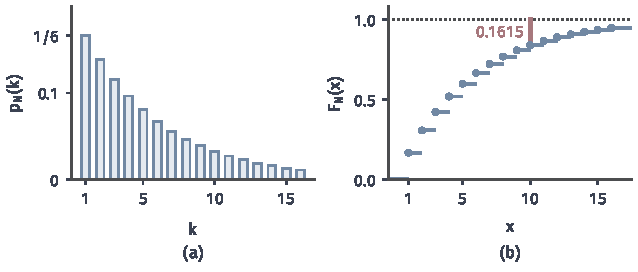
\includegraphics[width=108mm]{figures/07-probability/01-elementary-probability/matplotlib/rvd-first-six/figure.pdf}
  \caption{首次掷出六点所需次数$N$。(a)质量函数$p_N(k)=(5/6)^{k-1}/6$，只画出$k\leq16$；(b)分布函数$F_N$，在每个正整数处跳跃，点线是高度$1$。红线是$x=10$处尚未累计的质量$(5/6)^{10}\approx0.1615$。}
  \label{fig:rvd-first-six}
\end{BookInlineFigure}

\paragraph{核对一张概率表}
给出一张表时，要检查非负、总和为$1$，并说明支撑。设$X$取正整数，$p_X(k)=c/(k(k+1))$，常数$c$待定。把每一项拆成两个分数之差，部分和中间各项依次抵消：
\[
  \sum_{k=1}^{n}\frac{1}{k(k+1)}=\sum_{k=1}^{n}\Bigl(\frac1k-\frac1{k+1}\Bigr)=1-\frac1{n+1}.
\]
令$n\to\infty$，级数和为$1$，所以$c=1$。用同样的抵消，$\mathbb{P}(X\geq5)=1/5$，$F_X(k)=k/(k+1)$。这张表下一节还会用到：它的尾部衰减得很慢。

\paragraph{密度：单位长度上的概率}
等待时间的分布函数处处连续。对任意$t$和$h>0$，$\{T=t\}\subseteq\{t-h<T\leq t\}$，所以$\mathbb{P}(T=t)\leq F_T(t)-F_T(t-h)$，令$h\to0$即得$\mathbb{P}(T=t)=0$。每个单点的概率都是$0$，质量函数恒为零，提供不了任何信息。概率并没有消失，只是不再集中在一个个点上，而是像一根粗细不均的细棒上的质量那样沿实轴连续铺开。描述细棒，我们用线密度，即单位长度上的质量；某一段的质量是线密度在这一段上的积分。

先看一个能直接算出“单位长度上的概率”的例子。在半径为$1$的圆盘内随机取一点，规定点落在任一区域的概率等于该区域面积与圆盘面积$\pi$之比。记点到圆心的距离为$R$。$\{R\leq r\}$是半径$r$的小圆盘（图~\ref{fig:rvd-disk-radius}(a)），所以
\[
  F_R(r)=\frac{\pi r^{2}}{\pi}=r^{2},\qquad 0\leq r\leq1 .
\]
$r<0$时$F_R(r)=0$，$r>1$时$F_R(r)=1$。

\begin{BookInlineFigure}
  \centering
  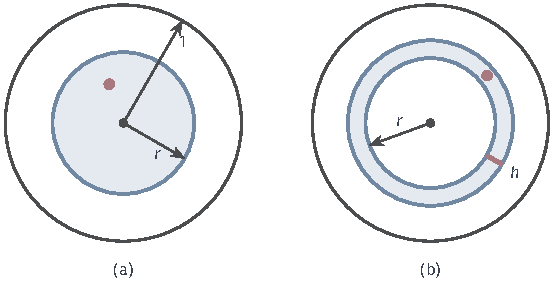
\includegraphics[width=94mm]{figures/07-probability/01-elementary-probability/tikz/rvd-disk-radius/figure.pdf}
  \caption{单位圆盘内随机取点（红点），$R$是它到圆心的距离。(a)事件$\{R\leq r\}$是浅蓝的小圆盘，概率为面积比$r^{2}$；(b)事件$\{r<R\leq r+h\}$是宽$h$的圆环，面积$\pi(2rh+h^{2})$，概率约为$2rh$。圆环越靠外越长，所以同样宽度的圆环外侧概率更大。}
  \label{fig:rvd-disk-radius}
\end{BookInlineFigure}

现在取一个宽$h$的圆环$\{r<R\leq r+h\}$（图~\ref{fig:rvd-disk-radius}(b)）。由式~\eqref{eq:rvd-interval}，
\[
  \mathbb{P}(r<R\leq r+h)=(r+h)^{2}-r^{2}=2rh+h^{2}.
\]
除以宽度$h$，得到这一段上平均每单位长度的概率：
\[
  \frac{\mathbb{P}(r<R\leq r+h)}{h}=2r+h .
\]
令$h\to0$，极限是$2r$。这就是$R$在$r$处的“单位长度上的概率”。

图~\ref{fig:rvd-density-histogram}把这个比值画成柱：每根柱的面积等于对应区间的概率，柱高是概率除以宽度。宽度从$0.25$缩小到$0.05$，柱顶越来越贴近直线$2r$。点在圆盘内是“均匀”取的，$R$却不均匀：离圆心越远，同样宽度的圆环越长，分到的概率越多。

\begin{BookInlineFigure}
  \centering
  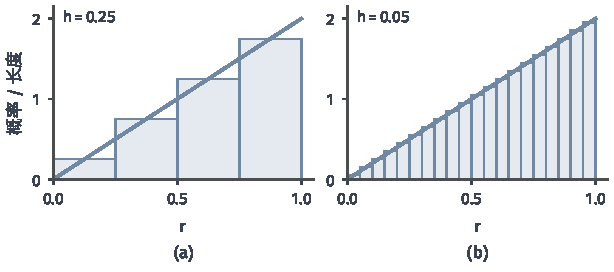
\includegraphics[width=104mm]{figures/07-probability/01-elementary-probability/matplotlib/rvd-density-histogram/figure.pdf}
  \caption{圆盘半径$R$的单位长度概率。浅蓝柱的宽度为$h$，高度为$\mathbb{P}(r<R\leq r+h)/h=2r+h$，面积就是该段的概率；蓝线是极限$2r$。(a)$h=0.25$；(b)$h=0.05$，柱顶与直线的差距缩小为$h$。}
  \label{fig:rvd-density-histogram}
\end{BookInlineFigure}

把这种描述作为定义：不再从分布函数出发求变化率，而是直接用一个函数的积分规定区间概率。

\begin{definition}[概率密度函数]
\label{def:rvd-density}
若存在非负函数$f_X$，使$\int_{-\infty}^{\infty}f_X(x)\,\mathrm{d}x=1$，并且对一切$a<b$都有
\begin{equation}
  \mathbb{P}(a<X\leq b)=\int_{a}^{b}f_X(x)\,\mathrm{d}x,
  \label{eq:rvd-density}
\end{equation}
就称$X$有\term{概率密度函数}（probability density function）$f_X$，简称密度。其中$a$可以取$-\infty$，$b$可以取$+\infty$，积分可以是反常积分。
\end{definition}

这里的积分是卷一意义下的黎曼积分，在无穷区间或被积函数无界时按反常积分理解，可参考\BookChapterRef{chap:univariate-integration}{卷一第7章“一元函数的积分”}。密度为正的范围称为它的支撑，例如$R$的支撑是$[0,1]$，等待时间的支撑是$[0,\infty)$。取$a=-\infty$，定义直接给出分布函数是密度的累计：
\begin{equation}
  F_X(x)=\int_{-\infty}^{x}f_X(t)\,\mathrm{d}t .
  \label{eq:rvd-cdf-from-density}
\end{equation}

\paragraph{密度模型的分布函数}
上一节对离散变量证明了分布函数的性质，现在对有密度的变量核验同样的性质，并看清单点概率为什么都是零。

\begin{theorem}[有密度时的分布函数]
\label{thm:rvd-density-cdf}
设$X$有密度$f_X$。则$F_X$单调不减、处处连续，$\lim_{x\to-\infty}F_X(x)=0$，$\lim_{x\to+\infty}F_X(x)=1$，并且对每个$x$都有$\mathbb{P}(X=x)=0$。若$f_X$在$x_0$处连续，则$F_X$在$x_0$处可导，且
\begin{equation}
  F_X'(x_0)=f_X(x_0).
  \label{eq:rvd-density-derivative}
\end{equation}
\end{theorem}

\begin{proof}
单调性来自被积函数非负：$x<y$时$F_X(y)-F_X(x)=\int_x^yf_X\geq0$。两端极限是反常积分$\int_{-\infty}^{\infty}f_X=1$收敛的定义：上限趋于$-\infty$时积分趋于$0$，趋于$+\infty$时积分趋于$1$。

连续性要证明$h\to0$时$\int_x^{x+h}f_X\to0$（$h<0$时理解为$-\int_{x+h}^{x}f_X$）。若$f_X$在$x$附近有界，设$\lvert f_X\rvert\leq K$，则这个积分的绝对值不超过$K\lvert h\rvert$，趋于$0$。若$f_X$在$x$附近无界，$x$是反常积分的瑕点，而反常积分收敛的定义正是积分上限（或下限）趋于瑕点时积分有极限，这个极限就是$F_X(x)$，所以积分同样趋于$0$。

单点概率：对$h>0$，$\{X=x\}\subseteq\{x-h<X\leq x\}$，于是
\[
  0\leq\mathbb{P}(X=x)\leq F_X(x)-F_X(x-h).
\]
由连续性，右边随$h\to0$趋于$0$，所以$\mathbb{P}(X=x)=0$。最后，$f_X$在$x_0$处连续时，式~\eqref{eq:rvd-density-derivative}是微积分基本定理对积分上限函数的结论。
\end{proof}

于是有密度的变量取任何一个具体值的概率都是$0$，而它每次总会取到某个值。这并不矛盾：实轴上有不可数多个点，概率是在区间上累计起来的，不是逐点相加起来的。“概率为零”与“不可能”在这里分开了：$\{T=1\}$是可能发生的事件，概率却为零。实际计算中的直接后果是端点开闭不再重要：
\[
  \mathbb{P}(a<X\leq b)=\mathbb{P}(a\leq X\leq b)=\mathbb{P}(a<X<b)=\int_a^bf_X(x)\,\mathrm{d}x .
\]

\paragraph{等待时间的密度}
式~\eqref{eq:rvd-waiting-cdf}的分布函数在$t\neq0$处可导，导数在$t<0$时为$0$，在$t>0$时为$\mathrm{e}^{-t}$。下面会说明，这样的分布函数由导数给出密度：
\[
  f_T(t)=\begin{cases}0,&t<0,\\\mathrm{e}^{-t},&t\geq0.\end{cases}
\]
图~\ref{fig:rvd-waiting-density-cdf}用两种方式表示同一个概率$\mathbb{P}(1<T\leq2)\approx0.2325$：在密度图中它是曲线下的面积，在分布函数图中它是两个函数值的高度差。密度越大的地方，分布函数上升越快。

\begin{BookInlineFigure}
  \centering
  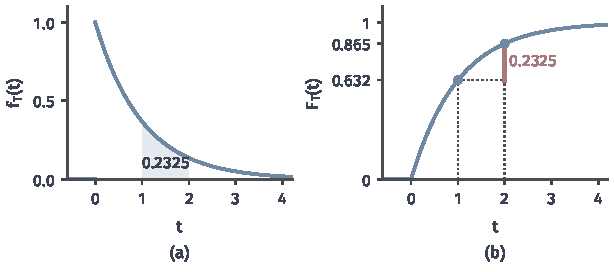
\includegraphics[width=104mm]{figures/07-probability/01-elementary-probability/matplotlib/rvd-waiting-density-cdf/figure.pdf}
  \caption{等待时间$T$的密度与分布函数。(a)密度$f_T(t)=\mathrm{e}^{-t}$（$t\geq0$），浅蓝面积是$\mathbb{P}(1<T\leq2)=\mathrm{e}^{-1}-\mathrm{e}^{-2}\approx0.2325$；(b)分布函数$F_T(t)=1-\mathrm{e}^{-t}$，同一概率是$t=2$与$t=1$处函数值之差（红线）。}
  \label{fig:rvd-waiting-density-cdf}
\end{BookInlineFigure}

\paragraph{由分布函数求密度}
定理~\ref{thm:rvd-density-cdf}说密度是分布函数的导数。反过来，什么时候能对分布函数求导得到密度？最常用的是下面这个充分条件。

\begin{theorem}[由分布函数求密度]
\label{thm:rvd-cdf-to-density}
设$F_X$处处连续，并且除有限个点$c_1<\dots<c_m$外连续可导，导数$F_X'$在每个开区间$(c_{k},c_{k+1})$上反常可积。令$f(x)=F_X'(x)$（在$c_k$处任意取非负值），则$f$是$X$的密度。
\end{theorem}

\begin{proof}
分布函数单调不减，所以导数$F_X'\geq0$，$f$非负。取$a<b$，在$a,b$之间插入落在其中的那些$c_k$，把$[a,b]$分成若干段。在每一段的内部，$F_X$连续可导，由Newton--Leibniz公式，$F_X$在段内两点之间的增量等于导数的积分；让两点趋于段端，$F_X$的连续性保证增量趋于整段的增量，积分按反常积分收敛到整段的积分。各段相加，得到
\[
  F_X(b)-F_X(a)=\int_a^bf(x)\,\mathrm{d}x .
\]
这就是式~\eqref{eq:rvd-density}。令$a\to-\infty$、$b\to+\infty$，由分布函数的两端极限得到$\int_{-\infty}^{\infty}f=1$。有限个点处的取值不影响积分。
\end{proof}

圆盘半径$R$满足条件：$F_R$连续，除$r=0,1$外可导，于是$f_R(r)=2r$（$0<r<1$），其余处为$0$，正是前面由圆环得到的极限。用它验算：
\[
  \mathbb{P}(0.5<R\leq1)=\int_{0.5}^{1}2r\,\mathrm{d}r=1-0.25=0.75 .
\]
从分布函数直接算是$F_R(1)-F_R(0.5)=0.75$，两者一致。条件中的“连续”不能去掉：抽检次品数的分布函数除三个点外导数都是零，按导数得到的“密度”积分为$0$，丢掉了全部质量。第~\ref{sec:rvd-representation-limits}节还会看到，即使分布函数连续，也可能求不出密度。

\paragraph{密度值不是概率}
密度的单位是“概率每单位长度”，它的值本身不是任何事件的概率。若$f_X$在$x$处连续，由积分中值定理，存在$\xi_h\in[x,x+h]$使
\[
  \mathbb{P}(x<X\leq x+h)=f_X(\xi_h)\,h\approx f_X(x)\,h .
\]
所以只有乘上一小段长度，密度才变成概率。密度的值可以大于$1$，甚至可以无界，只要曲线下的总面积是$1$。

图~\ref{fig:rvd-density-values}给出三个例子。(a)在$(0,1/2)$上$f(x)=2$，其余处为$0$，总面积$2\times\frac12=1$，而
\[
  \mathbb{P}(0.1<X\leq0.3)=2\times0.2=0.4 .
\]
(b)在$(0,1)$上$f(x)=6x(1-x)$，最大值$f(1/2)=1.5$，下面还会用它演示怎样核对密度。(c)在$(0,1]$上$f(x)=1/(2\sqrt{x})$，在$0$附近无界，但反常积分收敛，分布函数是$F(x)=\sqrt{x}$（$0\leq x\leq1$），于是
\[
  \mathbb{P}(X\leq\tfrac14)=\sqrt{1/4}=\tfrac12 .
\]

\begin{BookInlineFigure}
  \centering
  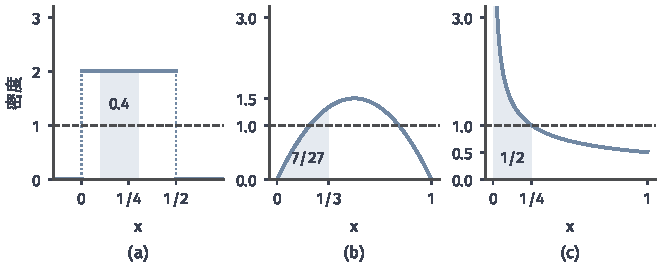
\includegraphics[width=112mm]{figures/07-probability/01-elementary-probability/matplotlib/rvd-density-values/figure.pdf}
  \caption{密度的高度不是概率。虚线是高度$1$，浅蓝面积是所标的概率。(a)$(0,1/2)$上的常数密度$2$，$\mathbb{P}(0.1<X\leq0.3)=0.4$；(b)$6x(1-x)$，最大值$1.5$，$\mathbb{P}(X\leq1/3)=7/27$；(c)$1/(2\sqrt{x})$在$0$附近无界，$\mathbb{P}(X\leq1/4)=1/2$。}
  \label{fig:rvd-density-values}
\end{BookInlineFigure}

密度值还依赖于单位。等待时间以分钟计时密度在$0$处等于$1$；改以小时计，$H=T/60$，于是对$s\geq0$，
\[
  \mathbb{P}(H\leq s)=\mathbb{P}(T\leq60s)=1-\mathrm{e}^{-60s}.
\]
求导得
\[
  f_H(s)=60\,\mathrm{e}^{-60s},\qquad s\geq0,
\]
在$0$处等于$60$。同一事件的概率不随单位改变，单位长度上的概率却要按长度单位换算。

\paragraph{核对一个函数是不是密度}
给出候选密度时，要核对三件事：在支撑上非负，总积分为$1$，支撑写清楚。设$f(x)=c\,x(1-x)$（$0<x<1$），其余处为$0$。在$(0,1)$上$x(1-x)>0$，非负性只要求$c>0$。归一化要求
\[
  c\int_0^1x(1-x)\,\mathrm{d}x=c\Bigl(\frac12-\frac13\Bigr)=\frac c6=1,
\]
所以$c=6$，这就是图~\ref{fig:rvd-density-values}(b)。它的分布函数是
\[
  F(x)=\int_0^x6t(1-t)\,\mathrm{d}t=3x^{2}-2x^{3},\qquad 0\leq x\leq1,
\]
所以$\mathbb{P}(X\leq1/3)=3/9-2/27=7/27\approx0.259$。

支撑不能随意扩大。若把同一公式用在$(0,2)$上，$1<x<2$时$x(1-x)<0$，无论$c$取什么正数都违反非负性；把公式写成“$f(x)=6x(1-x)$”而不写支撑，读者就无从判断它在区间外是什么。

\paragraph{从细格上的质量到密度}
质量与密度的关系可以通过把格子越分越细看出来。设$X_n$以概率$1/n$取$1/n,2/n,\dots,n/n$中的每一个值，相邻取值相距$1/n$。每一点的质量$1/n$随$n$增大趋于$0$，但质量除以格宽始终是
\[
  \frac{1/n}{1/n}=1 .
\]
分布函数是$F_{X_n}(x)=\lfloor nx\rfloor/n$（$0\leq x\leq1$），它与$x$的差不超过$1/n$。

当$n\to\infty$时，阶梯越来越密、台阶越来越矮，分布函数逼近$F(x)=x$，这正是$(0,1)$上常数密度$1$的分布函数。质量函数的值趋于零，提供不了极限的信息；分布函数和“质量除以格宽”却都有好的极限。所以比较离散与连续的模型时，要拿分布函数比，或者拿“质量/格宽”与密度比，不能拿单点质量与密度值比。分布怎样在这种意义下逼近，在第~\ref{chap:random-variable-convergence}章系统研究。

\paragraph{密度只在积分意义下确定}
改变$f_X$在有限个点处的值，所有区间上的积分都不变，因而规定的是同一个分布。所以“$X$的密度”实际上指一族只在有限个点处不同的函数，我们总选其中最方便的一个，例如在支撑的端点处取什么值都可以。与此不同，质量函数在每一点的值都有意义，改动任何一点都会改变分布。这也说明密度在单点上的值不能单独解释，只有它在小区间上的平均才对应概率。

表~\ref{tab:rvd-mass-vs-density}对比了两种表示。

\begin{BookInlineTable}
  \centering
  \begin{tabular}{lll}
    \toprule
    & 质量函数$p_X$ & 密度$f_X$\\
    \midrule
    区间概率 & 对取值求和 & 在区间上积分\\
    函数值 & 单点概率，不超过$1$ & 单位长度的概率，可大于$1$\\
    单点概率 & $p_X(x)$ & 恒为$0$\\
    分布函数 & 阶梯，跳跃高度为$p_X$ & 连续，导数为$f_X$\\
    端点开闭 & 可能改变结果 & 不影响结果\\
    改动一点的值 & 改变分布 & 不改变分布\\
    \bottomrule
  \end{tabular}
  \caption{概率质量函数与概率密度函数的对比。两者都要求非负、总量为$1$；区别在于质量集中在可数个点上，还是沿实轴连续铺开。}
  \label{tab:rvd-mass-vs-density}
\end{BookInlineTable}

习惯上把有密度的分布称为连续分布，把离散随机变量的分布称为离散分布。“连续分布”这个名字只说明分布函数连续；第~\ref{sec:rvd-representation-limits}节会看到，分布函数连续并不保证密度存在。


\section{分位数}
\label{sec:rvd-quantiles}

窗口想承诺“九成顾客的等待不超过某个时长”，这个时长应当定为多少？分布函数回答的是“给定阈值，累计概率多大”，现在的问题方向相反：给定累计概率$p$，求阈值$x$。

\paragraph{反解分布函数}
对等待时间，$F_T(t)=1-\mathrm{e}^{-t}$在$t\geq0$上连续且严格递增，方程$F_T(t)=p$对每个$0<p<1$恰有一个解：
\[
  1-\mathrm{e}^{-t}=p\quad\Longleftrightarrow\quad t=-\ln(1-p).
\]
取$p=0.9$，得$t=\ln10\approx2.303$分钟：九成顾客等待不超过约$2.3$分钟。

离散变量就没有这么顺利。公平骰子的分布函数在$[2,3)$上等于$1/3$，在$3$处跳到$1/2$，方程$F(x)=0.4$根本没有解；而$F(x)=1/2$对$[3,4)$中的每个$x$都成立，解有无穷多个。跳跃使某些$p$取不到，平台使某些$p$的解不唯一。我们需要一个对任何分布函数都有意义的约定。

自然的想法是不再要求“恰好等于$p$”，而是找累计概率首次达到$p$的位置。$p=0.4$时，阈值从左向右移动，到$x=3$时累计概率从$1/3$跳到$1/2$，第一次不小于$0.4$，所以取$3$。$p=1/2$时，累计概率在$x=3$处第一次达到$1/2$，平台上的其余点都在它右边，所以也取$3$。

\begin{definition}[分位数]
\label{def:rvd-quantile}
设$F$是随机变量$X$的分布函数，$0<p<1$。称
\begin{equation}
  Q(p)=\inf\{x\in\mathbb{R}:F(x)\geq p\}
  \label{eq:rvd-quantile}
\end{equation}
为$X$的$p$\term{分位数}（quantile），函数$p\mapsto Q(p)$称为\term{分位数函数}（quantile function）。$Q(1/2)$称为\term{中位数}（median），$Q(1/4)$与$Q(3/4)$分别称为下、上\term{四分位数}（quartile）。
\end{definition}

\paragraph{分位数与分布函数的对应}
分位数用到的只是分布函数的三条性质：单调不减、右连续、两端极限为$0$和$1$。前面各节的离散模型和密度模型都满足它们。下面的引理把下确界化成一个可以直接使用的等价关系。

\begin{lemma}[分位数的等价刻画]
\label{lem:rvd-quantile-galois}
设$0<p<1$。则$Q(p)$是有限实数，并且对一切实数$x$，
\begin{equation}
  Q(p)\leq x\quad\Longleftrightarrow\quad p\leq F(x).
  \label{eq:rvd-quantile-galois}
\end{equation}
\end{lemma}

\begin{proof}
记$A_p=\{x:F(x)\geq p\}$。因为$F(x)\to1>p$（$x\to+\infty$），$A_p$非空；因为$F(x)\to0<p$（$x\to-\infty$），$A_p$有下界。所以下确界$Q(p)$是有限实数。

$A_p$向右封闭：若$x\in A_p$且$y>x$，由单调性$F(y)\geq F(x)\geq p$，所以$y\in A_p$。再看下确界本身是否属于$A_p$。取$A_p$中的点列$x_n$从右侧趋于$Q(p)$，由右连续，
\[
  F(Q(p))=\lim_{n\to\infty}F(x_n)\geq p .
\]
所以$Q(p)\in A_p$，从而$A_p=[Q(p),\infty)$。“$x\in A_p$”就是“$p\leq F(x)$”，“$x\in[Q(p),\infty)$”就是“$Q(p)\leq x$”，二者等价。
\end{proof}

右连续在这里起了关键作用：它保证下确界被取到，集合$A_p$是带左端点的闭半直线。由引理可以读出分位数处的累计概率。取$x=Q(p)$，得$F(Q(p))\geq p$；对$x<Q(p)$有$F(x)<p$，令$x\uparrow Q(p)$，得左极限$F(Q(p)^{-})\leq p$。由式~\eqref{eq:rvd-jump}，这两条合起来是
\begin{equation}
  \mathbb{P}(X<Q(p))\leq p\leq\mathbb{P}(X\leq Q(p)).
  \label{eq:rvd-quantile-sandwich}
\end{equation}
也就是说，严格小于$p$分位数的概率至多是$p$，不超过它的概率至少是$p$。分布函数在$Q(p)$处连续时，两边相等，$F(Q(p))=p$。

\paragraph{平台与跳跃互换}
公平骰子的分位数函数可以直接写出。$F(x)=k/6$对$k\leq x<k+1$成立，由式~\eqref{eq:rvd-quantile-galois}，$Q(p)\leq k$当且仅当$p\leq k/6$，所以
\[
  Q(p)=k,\qquad \frac{k-1}{6}<p\leq\frac k6,\quad k=1,\dots,6 .
\]
特别地$Q(0.4)=3$，中位数$Q(1/2)=3$。图~\ref{fig:rvd-quantile-dice}把分布函数和分位数函数并排画出。

\begin{BookInlineFigure}
  \centering
  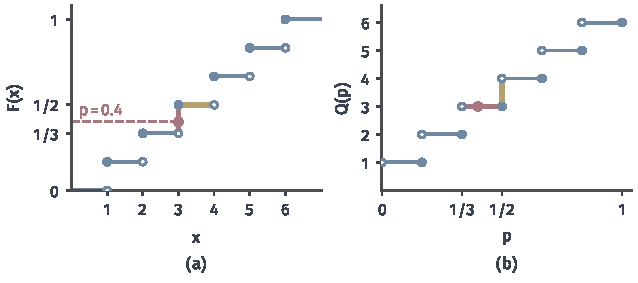
\includegraphics[width=108mm]{figures/07-probability/01-elementary-probability/matplotlib/rvd-quantile-dice/figure.pdf}
  \caption{公平骰子的分布函数与分位数函数。(a)分布函数，红色竖线是$x=3$处从$1/3$到$1/2$的跳跃，红色虚线$p=0.4$落在跳跃之内；黄线是高度$1/2$的平台$[3,4)$。(b)分位数函数，跳跃变成$(1/3,1/2]$上的平台（红线），红点是$Q(0.4)=3$；平台变成$p=1/2$处从$3$到$4$的跳跃（黄线）。实心点在每段右端，表示$Q$在跳跃点取左侧的值。}
  \label{fig:rvd-quantile-dice}
\end{BookInlineFigure}

图中可以看出两者的对偶。分布函数在$x=3$处跳跃$1/6$，累计概率在$(1/3,1/2]$中的所有$p$都“首次达到”于同一个位置$3$，于是分位数函数在这一段上是平台。分布函数在$[3,4)$上是平台，说明这一段没有质量，$p$稍大于$1/2$时阈值必须越过整段平台才能累计到更多概率，于是分位数函数在$p=1/2$处跳跃。几何上，分位数函数的图像就是把分布函数的图像沿对角线翻转，再在跳跃处按约定取左侧的值。

分位数函数单调不减，这由式~\eqref{eq:rvd-quantile}中集合$A_p$随$p$增大而缩小得到。它还是左连续的：设$p_n\uparrow p$，则$Q(p_n)$单调不减且不超过$Q(p)$，有极限$L\leq Q(p)$。对每个$n$有$Q(p_n)\leq L$，由引理$p_n\leq F(L)$；令$n\to\infty$得$p\leq F(L)$，再由引理$Q(p)\leq L$。所以$L=Q(p)$。分布函数右连续，分位数函数左连续，这是同一个约定的两面。

表~\ref{tab:rvd-cdf-vs-quantile}把两个函数的对应关系列在一起。

\begin{BookInlineTable}
  \centering
  \begin{tabular}{lll}
    \toprule
    & 分布函数$F$ & 分位数函数$Q$\\
    \midrule
    输入与输出 & 阈值$x\mapsto$累计概率 & 累计概率$p\mapsto$阈值\\
    定义域 & 全体实数 & $(0,1)$\\
    连续性约定 & 右连续 & 左连续\\
    跳跃 & 单点上的质量 & 一段没有质量的区间\\
    平台 & 一段没有质量的区间 & 单点上的质量\\
    \bottomrule
  \end{tabular}
  \caption{分布函数与分位数函数的对应。二者由式~\eqref{eq:rvd-quantile-galois}联系，一方的跳跃对应另一方的平台。}
  \label{tab:rvd-cdf-vs-quantile}
\end{BookInlineTable}

\paragraph{几个模型的分位数}
抽检次品数的分布函数是式~\eqref{eq:rvd-inspection-cdf}。用同样的方法读出
\[
  Q(p)=\begin{cases}0,&0<p\leq0.3,\\1,&0.3<p\leq0.9,\\2,&0.9<p<1.\end{cases}
\]
中位数是$1$：不超过$1$件次品的概率是$0.9$，严格少于$1$件的概率是$0.3$，两者把$1/2$夹在中间，与式~\eqref{eq:rvd-quantile-sandwich}一致。

等待时间的分位数函数是$Q(p)=-\ln(1-p)$。中位数和两个四分位数分别是
\[
  Q(\tfrac12)=\ln2\approx0.693,\quad Q(\tfrac14)=\ln\tfrac43\approx0.288,\quad Q(\tfrac34)=\ln4\approx1.386 .
\]
半数顾客等待不到$0.7$分钟，中间一半顾客的等待落在约$0.29$到$1.39$分钟之间。两个四分位数之差$Q(3/4)-Q(1/4)$称为\term{四分位距}（interquartile range），这里等于$\ln3\approx1.099$分钟，它从位置的角度衡量取值的分散程度。

另两个模型的分位数也有直接的含义。圆盘中随机点到圆心的距离满足$F_R(r)=r^{2}$，解得$Q(p)=\sqrt{p}$，中位数$\sqrt{1/2}\approx0.707$：一半的点落在半径约$0.707$的圆之外，因为这个圆的面积恰是整个圆盘的一半。

首次掷出六点所需的次数$N$满足$F_N(k)=1-(5/6)^{k}$。由式~\eqref{eq:rvd-quantile-galois}，$Q(p)\leq k$当且仅当$(5/6)^{k}\leq1-p$，即$k\geq\ln(1-p)/\ln(5/6)$，所以$Q(p)$是不小于$\ln(1-p)/\ln(5/6)$的最小正整数。算两个值：
\[
  F_N(3)=1-\tfrac{125}{216}\approx0.4213,\qquad F_N(4)=1-\tfrac{625}{1296}\approx0.5177 .
\]
累计概率在$k=4$时首次超过$1/2$，中位数是$4$。取$p=0.9$，$\ln0.1/\ln(5/6)\approx12.63$，于是$Q(0.9)=13$：要有九成把握见到六点，得准备掷$13$次。

\paragraph{平台上的中位数}
平台意味着一段没有质量的区间。设某服务只在两个时段开放，到达时刻$X$（单位：小时）在$[0,1]$与$[2,3]$上各以一半的概率均匀分布，即密度在这两段上为$1/2$，其余处为$0$。由式~\eqref{eq:rvd-cdf-from-density}，
\[
  F(x)=\begin{cases}x/2,&0\leq x\leq1,\\1/2,&1\leq x\leq2,\\(x-1)/2,&2\leq x\leq3,\end{cases}
\]
$x<0$时为$0$，$x>3$时为$1$。

图~\ref{fig:rvd-quantile-gap}显示，$F$在$[1,2]$上停在$1/2$。这一段的每个$m$都满足$\mathbb{P}(X\leq m)\geq1/2$且$\mathbb{P}(X\geq m)\geq1/2$，都把质量分成相等的两半。式~\eqref{eq:rvd-quantile}取其中最左的一个，$Q(1/2)=1$。也有书取平台的中点$1.5$，约定不同，但只有$F$在高度$p$处有平台时才会出现这种差别。

\begin{BookInlineFigure}
  \centering
  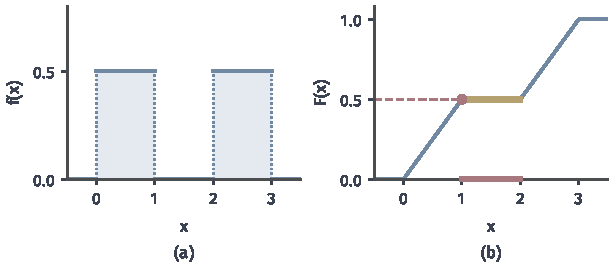
\includegraphics[width=104mm]{figures/07-probability/01-elementary-probability/matplotlib/rvd-quantile-gap/figure.pdf}
  \caption{密度有空档时的中位数。(a)密度在$[0,1]$与$[2,3]$上为$1/2$，中间为$0$；(b)分布函数在$[1,2]$上是高度$1/2$的平台（黄线），横轴上的红线$[1,2]$中每一点都把质量平分，红点是约定的中位数$Q(1/2)=1$。}
  \label{fig:rvd-quantile-gap}
\end{BookInlineFigure}

\paragraph{用二分法求分位数}
分布函数没有显式的反函数时，分位数要用数值方法求。引理~\ref{lem:rvd-quantile-galois}给出一个只用单调性的办法：对任意试探点$m$，计算$F(m)$并与$p$比较，$F(m)\geq p$说明$Q(p)\leq m$，否则$Q(p)>m$。每比较一次，就能把包含$Q(p)$的区间砍掉一半。这一判断不要求$F$连续或严格递增，跳跃和平台都不影响它。

以第~\ref{sec:rvd-mass-density}节的密度$6x(1-x)$为例，$F(x)=3x^{2}-2x^{3}$（$0\leq x\leq1$），求$0.9$分位数。中位数由对称性等于$1/2$，$0.9$分位数则要解三次方程$3x^{2}-2x^{3}=0.9$。从$[0,1]$出发，它一定包含$Q(0.9)$。每一轮取当前区间的中点$m$：若$F(m)\geq0.9$，把右端换成$m$；否则把左端换成$m$。前八轮的结果列在表~\ref{tab:rvd-bisection}中。

\begin{BookInlineTable}
  \centering
  \begin{tabular}{rllll}
    \toprule
    轮次 & 当前区间 & 中点$m$ & $F(m)$ & 判断\\
    \midrule
    1 & $[0,1]$ & $0.5$ & $0.5$ & $<0.9$，取右半\\
    2 & $[0.5,1]$ & $0.75$ & $0.8438$ & $<0.9$，取右半\\
    3 & $[0.75,1]$ & $0.875$ & $0.9570$ & $\geq0.9$，取左半\\
    4 & $[0.75,0.875]$ & $0.8125$ & $0.9077$ & $\geq0.9$，取左半\\
    5 & $[0.75,0.8125]$ & $0.78125$ & $0.8774$ & $<0.9$，取右半\\
    6 & $[0.78125,0.8125]$ & $0.796875$ & $0.8930$ & $<0.9$，取右半\\
    7 & $[0.796875,0.8125]$ & $0.8046875$ & $0.9005$ & $\geq0.9$，取左半\\
    8 & $[0.796875,0.8046875]$ & $0.80078125$ & $0.8967$ & $<0.9$，取右半\\
    \bottomrule
  \end{tabular}
  \caption{用二分法求$F(x)=3x^{2}-2x^{3}$的$0.9$分位数。每一轮区间长度减半，八轮后区间为$[0.80078125,0.8046875]$，长度$2^{-8}$。}
  \label{tab:rvd-bisection}
\end{BookInlineTable}

八轮之后，$Q(0.9)$被夹在$[0.80078,0.80469]$中，长度$2^{-8}\approx0.0039$。继续下去，区间收缩到$Q(0.9)\approx0.8042$。$k$轮之后区间长度是初始长度乘以$2^{-k}$，要达到精度$\varepsilon$只需约$\log_2(1/\varepsilon)$轮，每轮计算一次$F$。初始区间若未知，可以先向两侧加倍试探，直到找到$F(a)<p\leq F(b)$的两点。

\paragraph{分位数函数确定分布}
分位数函数是分布函数的广义逆，它是否也记下了全部信息？答案是肯定的，而且可以直接从引理~\ref{lem:rvd-quantile-galois}读出。对每个$x$，满足$Q(p)\leq x$的$p$恰是$(0,1)$中不超过$F(x)$的那些数，于是在$0<F(x)<1$时
\[
  F(x)=\max\{p\in(0,1):Q(p)\leq x\}.
\]
$F(x)=0$或$1$时，这个集合分别是空集或整个$(0,1)$，同样能读出$F(x)$。所以两个分布的分位数函数相同，它们的分布函数就相同。

还可以用分位数函数把一个最简单的随机变量变成任意给定分布的随机变量。设$U$有密度$1$（$0<u<1$），其余处为$0$，则$\mathbb{P}(U\leq u)=u$（$0\leq u\leq1$）。

\begin{theorem}[分位数变换]
\label{thm:rvd-quantile-transform}
设$F$是一个分布函数，$Q$是它的分位数函数，$U$如上。则$Q(U)$的分布函数是$F$。
\end{theorem}

\begin{proof}
$U$以概率$1$落在$(0,1)$中，那里$Q$有定义。对任意$x$，由引理~\ref{lem:rvd-quantile-galois}，$Q(U)\leq x$与$U\leq F(x)$是同一个事件，所以
\[
  \mathbb{P}(Q(U)\leq x)=\mathbb{P}(U\leq F(x))=F(x),
\]
最后一步用到$0\leq F(x)\leq1$。
\end{proof}

这个定理把“沿实轴均匀铺开的单位质量”按分位数函数重新安放：$U$落在$(1/3,1/2]$中的那一份质量，在骰子的例子中全部被送到$3$，于是$3$分到$1/6$的概率。

\paragraph{分位数与尾概率}
给定阈值$x$，事件$\{X>x\}$的概率$1-F(x)$称为$x$处的尾概率，它描述质量在$x$右侧的残余。给定小的比例$\alpha$，上侧分位数$Q(1-\alpha)$是“超过它的概率至多为$\alpha$”的最小阈值：由式~\eqref{eq:rvd-quantile-sandwich}，
\[
  \mathbb{P}\bigl(X>Q(1-\alpha)\bigr)=1-F\bigl(Q(1-\alpha)\bigr)\leq\alpha .
\]
尾概率和分位数是从两个方向读同一条曲线：前者由横轴读纵轴，后者由纵轴读横轴。

图~\ref{fig:rvd-quantile-tail}用等待时间演示。(a)从纵轴上的$0.5$和$0.9$出发读出中位数$\ln2$和$0.9$分位数$\ln10$。(b)画的是尾概率$1-F_T(t)=\mathrm{e}^{-t}$：从$t=1$读出$\mathbb{P}(T>1)=\mathrm{e}^{-1}\approx0.368$；在$t=\ln10$处尾概率恰为$0.1$，浅蓝面积就是这剩下的一成顾客。完整的分布已知时，两个方向都能精确计算；只知道分布的少数数值特征时，第~\ref{chap:tail-probabilities}章研究怎样给尾概率一个上界。

\begin{BookInlineFigure}
  \centering
  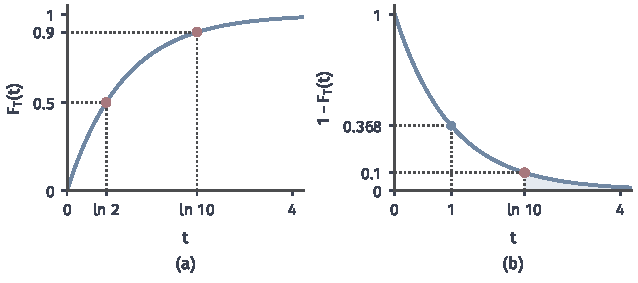
\includegraphics[width=108mm]{figures/07-probability/01-elementary-probability/matplotlib/rvd-quantile-tail/figure.pdf}
  \caption{等待时间的分位数与尾概率。(a)分布函数$1-\mathrm{e}^{-t}$，红点给出$Q(0.5)=\ln2$与$Q(0.9)=\ln10$；(b)尾概率$\mathrm{e}^{-t}$，蓝点是$t=1$处的$0.368$，红点是$t=\ln10$处的$0.1$，浅蓝区域表示超过$0.9$分位数的那部分。}
  \label{fig:rvd-quantile-tail}
\end{BookInlineFigure}

\paragraph{改变单位}
把等待时间从分钟换成秒，所有分位数都乘以$60$，这对一般的平移和正比例缩放都成立。设$a>0$，$b$为实数，$Y=aX+b$。对任意$y$，$\{Y\leq y\}=\{X\leq(y-b)/a\}$，所以$F_Y(y)=F_X((y-b)/a)$。由引理~\ref{lem:rvd-quantile-galois}，
\[
  Q_Y(p)\leq y\iff p\leq F_X\Bigl(\frac{y-b}{a}\Bigr)\iff Q_X(p)\leq\frac{y-b}{a}\iff aQ_X(p)+b\leq y .
\]
对一切$y$成立，于是$Q_Y(p)=aQ_X(p)+b$。$a<0$时不等号方向翻转，下侧分位数变成上侧，平台和跳跃处的约定也随之改变，需要另行处理。

\paragraph{描述位置而不是平均}
中位数和其他分位数描述的是分布的位置：取值在什么地方把质量按给定比例分开。它们只依赖取值的先后顺序和累计质量，不依赖远处的取值究竟有多远。

设$X$以概率$1/5$取$1,2,3,4,5$，中位数是$3$。把最大的取值$5$改成$12$，其余不变，$F$在$3$及其左侧不受影响，中位数仍是$3$。另一种描述中心的方式是按概率加权求和$\sum_xx\,p_X(x)$，下一章把它作为期望来研究。它同时看取值的大小，改动后从
\[
  \tfrac15(1+2+3+4+5)=3
\]
变为
\[
  \tfrac15(1+2+3+4+12)=4.4 .
\]
图~\ref{fig:rvd-median-shift}画出了这一对比：一个远处的取值就能把加权和拉过去，中位数却纹丝不动。

\begin{BookInlineFigure}
  \centering
  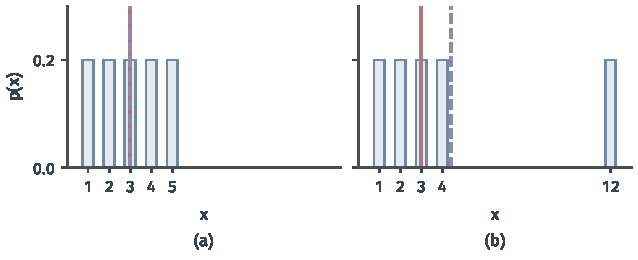
\includegraphics[width=108mm]{figures/07-probability/01-elementary-probability/matplotlib/rvd-median-shift/figure.pdf}
  \caption{中位数只看顺序。每个取值的概率都是$1/5$，红线是中位数$3$，紫色虚线是加权和$\sum_xx\,p_X(x)$。(a)取值$1,\dots,5$，两者都等于$3$；(b)把$5$移到$12$，中位数不变，加权和变为$4.4$。}
  \label{fig:rvd-median-shift}
\end{BookInlineFigure}

分位数还有一个优点：它对每个分布都存在。上一节的概率表$p_X(k)=1/(k(k+1))$有$F_X(1)=1/2$，所以中位数是$1$；而加权和
\[
  \sum_{k=1}^{\infty}k\cdot\frac{1}{k(k+1)}=\sum_{k=1}^{\infty}\frac{1}{k+1}
\]
是发散的调和级数，没有有限值。尾部质量衰减太慢时，加权平均会失去意义，分位数照样可以计算。至于什么时候加权平均存在、它与分位数各回答什么问题，在第~\ref{chap:random-variable-moments}章讨论。


\section{分布表示的边界}
\label{sec:rvd-representation-limits}

到目前为止，每个例子要么能列成一张概率表，要么有密度。是不是所有随机变量都属于这两类之一？先看一个很平常的等待问题，它两类都不属于。

\paragraph{有时不用等}
顾客来到窗口时，若窗口恰好空闲（概率$0.3$），等待时间为$0$；否则等待时间按式~\eqref{eq:rvd-waiting-cdf}的规律分布。记等待时间为$W$。由全概率公式，对$t\geq0$，
\[
  \mathbb{P}(W\leq t)=0.3\cdot1+0.7\,(1-\mathrm{e}^{-t}),
\]
其中第一项是窗口空闲、等待为$0$的情形，第二项是窗口忙、等待不超过$t$的情形。于是
\begin{equation}
  F_W(t)=\begin{cases}0,&t<0,\\0.3+0.7\,(1-\mathrm{e}^{-t}),&t\geq0.\end{cases}
  \label{eq:rvd-mixed-cdf}
\end{equation}
图~\ref{fig:rvd-mixed-cdfs}(a)画出了这条曲线：它在$0$处从$0$跳到$0.3$，之后连续上升。

\begin{BookInlineFigure}
  \centering
  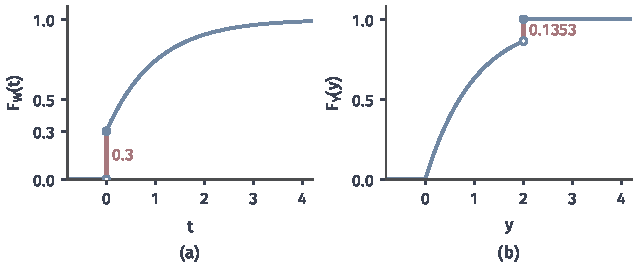
\includegraphics[width=108mm]{figures/07-probability/01-elementary-probability/matplotlib/rvd-mixed-cdfs/figure.pdf}
  \caption{既有跳跃又有连续上升的分布函数。(a)可能不用等的等待时间$W$，在$0$处跳跃$0.3$（红线），之后按$0.7(1-\mathrm{e}^{-t})$连续增加；(b)截断的等待时间$Y=\min\{T,2\}$，在$[0,2)$上与$1-\mathrm{e}^{-y}$相同，在$2$处跳跃$\mathrm{e}^{-2}\approx0.1353$。空心点是左极限，实心点是函数值。}
  \label{fig:rvd-mixed-cdfs}
\end{BookInlineFigure}

$W$不是离散随机变量。按模型，$0$这一点带有概率$0.3$；分布函数在其余各点连续，用第~\ref{sec:rvd-mass-density}节对等待时间所用的夹逼，其余每一点的概率都是$0$；可数个点上的质量加起来至多$0.3$，凑不满$1$。$W$也没有密度。若有密度，定理~\ref{thm:rvd-density-cdf}要求$\mathbb{P}(W=0)=0$，与$0.3$矛盾。概率表和密度都只能描述$W$的一部分质量。

计算时把两部分分开处理：跳跃部分求和，连续部分积分。对区间$B$，
\begin{equation}
  \mathbb{P}(W\in B)=0.3\cdot\mathbf{1}_{B}(0)+0.7\int_{B\cap(0,\infty)}\mathrm{e}^{-t}\,\mathrm{d}t,
  \label{eq:rvd-mixed-prob}
\end{equation}
其中$\mathbf{1}_{B}(0)$在$0\in B$时为$1$，否则为$0$。下面用三个区间演示。是否包含$0$决定了第一项：
\[
  \mathbb{P}(W\leq1)=0.3+0.7(1-\mathrm{e}^{-1})\approx0.7425,
\]
\[
  \mathbb{P}(0<W\leq1)=0.7(1-\mathrm{e}^{-1})\approx0.4425 .
\]
远离$0$的区间只有第二项，例如$\mathbb{P}(W>2)=0.7\,\mathrm{e}^{-2}\approx0.0947$。

分位数照样按式~\eqref{eq:rvd-quantile}计算。$p\leq0.3$时，$F_W(0)=0.3\geq p$而$t<0$时$F_W(t)=0$，所以$Q(p)=0$：有三成顾客根本不用等。$p>0.3$时解$0.3+0.7(1-\mathrm{e}^{-t})=p$，得
\[
  Q(p)=\ln\frac{0.7}{1-p},\qquad 0.3<p<1 .
\]
中位数是$\ln(7/5)\approx0.336$分钟，比不考虑空闲时的$\ln2\approx0.693$分钟短。

\paragraph{截断产生的跳跃}
这类分布并不罕见，对有密度的变量取函数就可能产生。设顾客最多等$2$分钟，等不到就离开，记录到的时长是$Y=\min\{T,2\}$。$y<2$时$\{Y\leq y\}=\{T\leq y\}$；$y\geq2$时$Y\leq y$总成立。所以
\[
  F_Y(y)=\begin{cases}0,&y<0,\\1-\mathrm{e}^{-y},&0\leq y<2,\\1,&y\geq2.\end{cases}
\]
它在$2$处跳跃，跳跃高度$\mathrm{e}^{-2}\approx0.1353$就是$\mathbb{P}(T\geq2)$：所有等待超过$2$分钟的质量都被堆到了$2$这一点上（图~\ref{fig:rvd-mixed-cdfs}(b)）。测量仪器有量程上限、记录有截止时间时，都会出现这种情形。

$Y$的分位数显示出跳跃的另一面。$p\leq1-\mathrm{e}^{-2}\approx0.8647$时，方程$1-\mathrm{e}^{-y}=p$在$[0,2)$中有解，$Q_Y(p)=-\ln(1-p)$，与$T$的分位数相同；$p>0.8647$时，累计概率在$y=2$处才首次达到$p$，$Q_Y(p)=2$。分布函数在$2$处的跳跃，变成了分位数函数在$(0.8647,1)$上的平台。截断只改变了高分位数，中位数仍是$\ln2$。

\paragraph{分离跳跃}
两个例子都由“跳跃部分”和“连续部分”组成。这种分离对任何分布函数都可以做到：先证明跳跃只能有可数个，再把它们集中成一张概率表，剩下的部分连续。

\begin{theorem}[分布函数的跳跃分解]
\label{thm:rvd-jump-decomposition}
设$F$单调不减、右连续，且$\lim_{x\to-\infty}F(x)=0$，$\lim_{x\to+\infty}F(x)=1$。记$J(a)=F(a)-F(a^{-})$为$a$处的跳跃高度。则
\begin{enumerate}
  \item 跳跃点$\{a:J(a)>0\}$至多可数，且跳跃高度的总和不超过$1$；
  \item 令
  \begin{equation}
    F_{\mathrm{d}}(x)=\sum_{a\leq x}J(a),\qquad F_{\mathrm{c}}(x)=F(x)-F_{\mathrm{d}}(x),
    \label{eq:rvd-jump-parts}
  \end{equation}
  则$F_{\mathrm{c}}$单调不减且处处连续。
\end{enumerate}
\end{theorem}

\begin{proof}
先看有限个跳跃点$a_1<a_2<\dots<a_m$。对相邻的两点，单调性给出$F(a_k)\leq F(a_{k+1}^{-})$，所以各段增量
\[
  F(a_m)-F(a_1^{-})=\sum_{k=1}^{m}J(a_k)+\sum_{k=1}^{m-1}\bigl(F(a_{k+1}^{-})-F(a_k)\bigr)\geq\sum_{k=1}^{m}J(a_k).
\]
左边不超过$1$，所以任意有限个跳跃高度之和不超过$1$。

固定正整数$n$。若有$m$个点的跳跃高度都大于$1/n$，则$m/n<1$，即$m<n$。所以跳跃高度大于$1/n$的点少于$n$个。全部跳跃点是这些有限集对$n=1,2,\dots$的并，因而至多可数；任意有限部分和不超过$1$，总和也不超过$1$。

再看$F_{\mathrm{c}}$。对$x<y$，把上面的论证用在$(x,y]$中有限个跳跃点上，再取上确界，得到
\[
  F(y)-F(x)\geq\sum_{x<a\leq y}J(a)=F_{\mathrm{d}}(y)-F_{\mathrm{d}}(x),
\]
即$F_{\mathrm{c}}(y)\geq F_{\mathrm{c}}(x)$。

$F_{\mathrm{d}}$与离散变量的分布函数结构相同：可数个点$a$各带非负质量$J(a)$，只是总量可能小于$1$。定理~\ref{thm:rvd-cdf-properties}中右连续与左极限的证明只用到质量非负、总和有限，所以$F_{\mathrm{d}}$右连续，并且在$a$处的跳跃恰为$J(a)$。$F$本身右连续、在$a$处跳跃$J(a)$，二者相减，$F_{\mathrm{c}}$右连续且在每点的跳跃为$0$，即处处连续。
\end{proof}

对$W$，$F_{\mathrm{d}}(t)=0.3\cdot\mathbf{1}_{\{t\geq0\}}$，连续部分在$t\geq0$时为$0.7(1-\mathrm{e}^{-t})$，它有密度$0.7\,\mathrm{e}^{-t}$，式~\eqref{eq:rvd-mixed-prob}正是按这一分解写成的。对$Y$，跳跃部分是$2$处的$\mathrm{e}^{-2}$，连续部分在$[0,2]$上由密度$\mathrm{e}^{-y}$积分得到。那么，连续部分是不是总有密度？

\paragraph{分布函数连续也未必有密度}
下面构造一个分布函数处处连续、却没有密度的随机变量。反复抛一枚公平硬币，各次独立，第$k$次正面记$D_k=1$，反面记$D_k=0$。令
\begin{equation}
  X=\sum_{k=1}^{\infty}\frac{2D_k}{3^{k}} .
  \label{eq:rvd-cantor}
\end{equation}
级数各项不超过$2/3^{k}$，总是收敛，$X\in[0,1]$。用三进制看，$X$的第$k$位小数是$2D_k$，只取$0$或$2$，永远不取$1$。

前$n$次抛掷决定了$X$落在哪一段。前$n$项的和是若干个$2/3^{k}$之和，剩余各项之和满足
\[
  0\leq\sum_{k>n}\frac{2D_k}{3^{k}}\leq\sum_{k>n}\frac{2}{3^{k}}=\frac{1}{3^{n}},
\]
所以$X$落在以前$n$项之和为左端点、长$3^{-n}$的闭区间里。前$n$次抛掷有$2^{n}$种等可能的结果，对应$2^{n}$个这样的区间，每个的概率是$2^{-n}$。

这些区间可以一层层画出来（图~\ref{fig:rvd-cantor-split}）。第一层是$[0,1/3]$和$[2/3,1]$，由$D_1=0$或$1$决定，各得一半质量；中间的$(1/3,2/3)$对应三进制首位为$1$，得不到任何质量。下一层把每个保留的区间再三等分，质量对半分给左右两段，中间一段又是空的。记第$n$层的$2^{n}$个区间之并为$C_n$，则$\mathbb{P}(X\in C_n)=1$，而$C_n$的总长度是$(2/3)^{n}$。

\begin{BookInlineFigure}
  \centering
  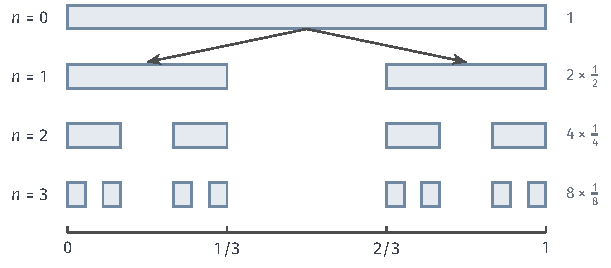
\includegraphics[width=104mm]{figures/07-probability/01-elementary-probability/tikz/rvd-cantor-split/figure.pdf}
  \caption{式~\eqref{eq:rvd-cantor}中$X$的质量怎样一层层分配。第$n$层有$2^{n}$个长$3^{-n}$的区间，每个区间的质量平分给它的左右两个三分之一，中间三分之一得不到质量。右侧是每层区间的个数与各自的质量；第$n$层总长$(2/3)^{n}$，总质量始终为$1$。}
  \label{fig:rvd-cantor-split}
\end{BookInlineFigure}

第一个结论：$F_X$处处连续。同一层的区间彼此之间至少隔着长$3^{-n}$的空档，所以长度小于$3^{-n}$的任何区间至多与该层的两个区间相交。对任意$x$和$0<h<3^{-n}/2$，区间$(x-h,x+h]$长度小于$3^{-n}$，于是
\[
  F_X(x+h)-F_X(x-h)=\mathbb{P}(x-h<X\leq x+h)\leq2\cdot2^{-n}.
\]
$n$可以任意大，所以$h\to0$时这个差趋于$0$，$F_X$在$x$处连续。特别地，每个单点的概率都是$0$，$X$不是离散随机变量。

第二个结论：$X$没有有界的密度。若$X$有密度$f$且$f\leq K$，则$X$落在$C_n$的概率是$f$在这$2^{n}$个区间上的积分之和，不超过$K$乘总长度：
\[
  1=\mathbb{P}(X\in C_n)\leq K\Bigl(\frac23\Bigr)^{n}.
\]
令$n\to\infty$，右边趋于$0$，矛盾。直观地说，全部质量挤在总长度任意小的集合上，单位长度上的概率只能无限大。

去掉“有界”这个限制，结论仍然成立：$X$根本没有密度。对无界的被积函数，上面的估计不再可用，严格证明需要比黎曼积分更一般的积分理论，可参考\BookChapterRef{chap:measure-densities}{卷四第8章“测度的密度”}。从分布函数一侧也能看到问题所在：$F_X$在被删去的每个中间三分之一上都是常数（那里没有质量），这些开区间的总长度是$1-(2/3)^{n}\to1$，所以$F_X$的导数在总长为$1$的范围内都是$0$；然而$F_X$从$0$升到了$1$。对导数积分只会得到$0$。定理~\ref{thm:rvd-cdf-to-density}的途径在这里失效，因为它要求除有限个点外可导。而对每一层都被保留的点$x$，包含$x$的第$n$层区间长$3^{-n}$，$F_X$在其上增加$2^{-n}$，差商为$(3/2)^{n}$，随$n$增大趋于无穷，所以$F_X$在这些点处不可导，这样的点有无穷多个。

图~\ref{fig:rvd-cantor-cdf}画出了$F_X$，它称为Cantor函数，$X$的分布称为\term{Cantor分布}（Cantor distribution）。黄线和紫线是把第$1$、$2$层的质量在各区间内均匀铺开得到的分布函数，蓝线是极限。每加细一层，上升的部分被压缩到更短的区间里，坡度变陡，平台变多。

\begin{BookInlineFigure}
  \centering
  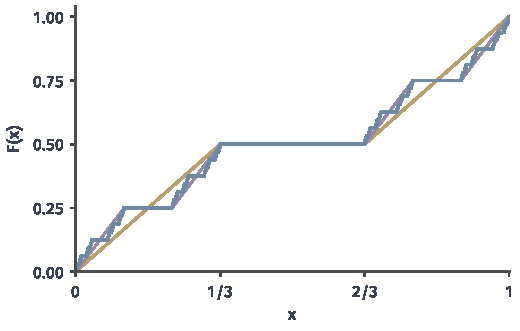
\includegraphics[width=88mm]{figures/07-probability/01-elementary-probability/matplotlib/rvd-cantor-cdf/figure.pdf}
  \caption{Cantor分布的分布函数（蓝线）。黄线与紫线分别把第$1$层、第$2$层区间上的质量均匀铺开，坡度为$(3/2)^{n}$。极限曲线连续，从$0$升到$1$，却在总长为$1$的一组区间上保持水平。}
  \label{fig:rvd-cantor-cdf}
\end{BookInlineFigure}

这个例子是专门构造出来的，在建模中很少直接出现。它说明的是一条边界：离散分布、有密度的分布以及二者的组合，并没有穷尽全部分布。一般的分布函数在去掉跳跃部分之后，连续部分还可以再分成有密度的部分和像Cantor函数这样没有密度的部分，相应的分解定理在卷四的同一章中给出。

\paragraph{各种表示的适用范围}
图~\ref{fig:rvd-representations}把本章的例子放到一起。分布函数对所有分布都存在；概率表只适用于离散分布；密度只适用于有密度的分布；像$W$和$Y$那样的分布需要两者组合；Cantor分布的分布函数连续，却两者都用不上。

\begin{BookInlineFigure}
  \centering
  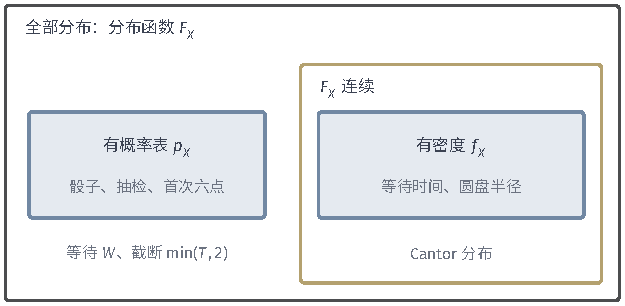
\includegraphics[width=105mm]{figures/07-probability/01-elementary-probability/tikz/rvd-representations/figure.pdf}
  \caption{各种表示的适用范围。外框是全部分布，它们都有分布函数；左侧蓝框是有概率表的离散分布，右侧黄框是分布函数连续的分布，其中蓝框是有密度的分布。框外标注的是两者都不适用的例子：可能不用等的$W$与截断的$\min\{T,2\}$既有跳跃又有连续部分，Cantor分布连续却没有密度。}
  \label{fig:rvd-representations}
\end{BookInlineFigure}

要对所有这些情形使用同一种语言，就不能再依赖“求和”与“黎曼积分”这两种具体的计算方式，而要直接把分布看作对实轴子集赋予概率的规则，并为它建立统一的积分。第~\ref{chap:probability-spaces}章完成这件事：概率表、密度以及它们的组合都成为同一种对象的特例，Cantor分布也能放进同一框架。在那之前，本部分只使用离散模型、密度模型以及按式~\eqref{eq:rvd-mixed-prob}那样分开计算的组合。


\section{本章小结}
\label{sec:rvd-summary}

本章从“由试验结果算出的数”出发。随机变量是样本空间上的函数，它把结果上的概率搬到实轴上，得到分布。分布只记录取值落在各处的概率，不记录这些取值来自哪个结果，所以同分布的变量可以在每次试验中取值完全不同，涉及几个变量之间关系的问题要留给随机向量。

分布有几种表示，各有成立的条件。分布函数$F_X(x)=\mathbb{P}(X\leq x)$对一切随机变量都有定义，单调不减、右连续、两端趋于$0$和$1$，跳跃高度是单点概率。概率质量函数只适用于离散变量，用求和计算概率；密度只适用于有密度的变量，用积分计算概率，它的值是单位长度上的概率，可以大于$1$，在有限个点处改动不影响分布。分位数$Q(p)=\inf\{x:F(x)\geq p\}$从反方向读分布函数，对一切分布都存在，并且与分布函数相互确定。

用可能不用等的等待时间$W$把这些表示串起来，可以看清各种表示分别用在哪里。分布函数由式~\eqref{eq:rvd-mixed-cdf}给出，任何区间的概率都能从它和它的左极限读出，例如$\mathbb{P}(W\leq1)\approx0.7425$。$W$在$0$处有$0.3$的质量，这部分只能用概率表描述；其余$0.7$的质量有密度$0.7\,\mathrm{e}^{-t}$，只能用积分描述；两者都不能单独代表整个分布。分位数在$p\leq0.3$时为$0$，中位数是$\ln(7/5)\approx0.336$分钟，它们描述的是质量按比例分开的位置。

表~\ref{tab:rvd-summary}汇总了各种表示。选用哪一种，先看分布属于哪一类，再看问题是给定范围求概率，还是给定概率求阈值。

\begin{BookInlineTable}
  \centering
  \begin{tabular}{lll}
    \toprule
    表示 & 适用范围 & 计算方式\\
    \midrule
    分布函数$F_X$ & 一切分布 & 相减，端点处用左极限\\
    质量函数$p_X$ & 离散分布 & 对取值求和\\
    密度$f_X$ & 有密度的分布 & 在区间上积分\\
    跳跃与密度组合 & 如$W$、$\min\{T,2\}$ & 跳跃求和，连续部分积分\\
    分位数$Q$ & 一切分布 & 给定概率反求阈值\\
    \bottomrule
  \end{tabular}
  \caption{分布的几种表示及其适用范围。Cantor分布的分布函数连续，却既无概率表也无密度，只能用分布函数或分位数函数描述。}
  \label{tab:rvd-summary}
\end{BookInlineTable}

这些表示的边界也要记住。分布函数连续不保证密度存在；一般情形下哪些集合可以赋予概率、分布函数为什么唯一确定分布，都在第~\ref{chap:probability-spaces}章统一建立。完整的分布包含全部概率规律，但使用起来往往太细。下一章从分布中提取平均位置和波动大小这样的少数数值，并说明它们存在的条件；中位数与加权平均的对比已经表明，几个数值只是分布的概括，不能代替分布本身。

